\section{Completion Level of Each Requirement}
\subsection{Self Assessment}
\subsubsection{Implementation of 5 core algorithms}
\begin{itemize}
    \item Breadth First Search (BFS): 10
    \item Depth First Search (DFS): 10
    \item Uniform-Cost Search (UCS): 
    \item Greedy Best First Search (GBFS): 10
    \item A* Search: 10
\end{itemize}
\subsubsection{Implementation of additional algorithms}
\begin{itemize}
    \item Iterative Deepening Search (IDS): 10
    \item A* with Manhattan Distance: 10
\end{itemize}
\subsection{5 test cases for each algorithm}

\subsubsection{test case 1}
\begin{figure}[h!]
    \centering
    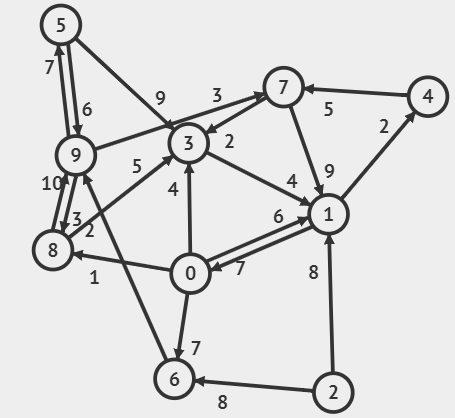
\includegraphics[width=0.5\textwidth]{testcase/1.PNG}
    \caption{Test Case 1 Image}
\end{figure}
\textbf{This is adjency matrix for test case 1.} 
\begin{verbatim}
2 5
0 6 0 4 0 0 7 0 1 0
7 0 0 0 2 0 0 0 0 0
0 8 0 0 0 0 8 0 0 0
0 4 0 0 0 0 0 0 0 0
0 0 0 0 0 0 0 5 0 0
0 0 0 9 0 0 0 0 0 6
0 0 0 0 0 0 0 0 0 2
0 9 0 2 0 0 0 0 0 0
0 0 0 5 0 0 0 0 0 10
0 0 0 0 0 7 0 3 3 0    
\end{verbatim}
\textbf{Test case Description:} 
\begin{itemize}
    \item Number of nodes: 10
    \item Number of edges: 20
    \item Start node: 2
    \item Goal node: 5
\end{itemize}

\paragraph*{Algorithm Results}
\quad The following are the results of the algorithms for test case 1.

\begin{figure}[h!]
    \centering
    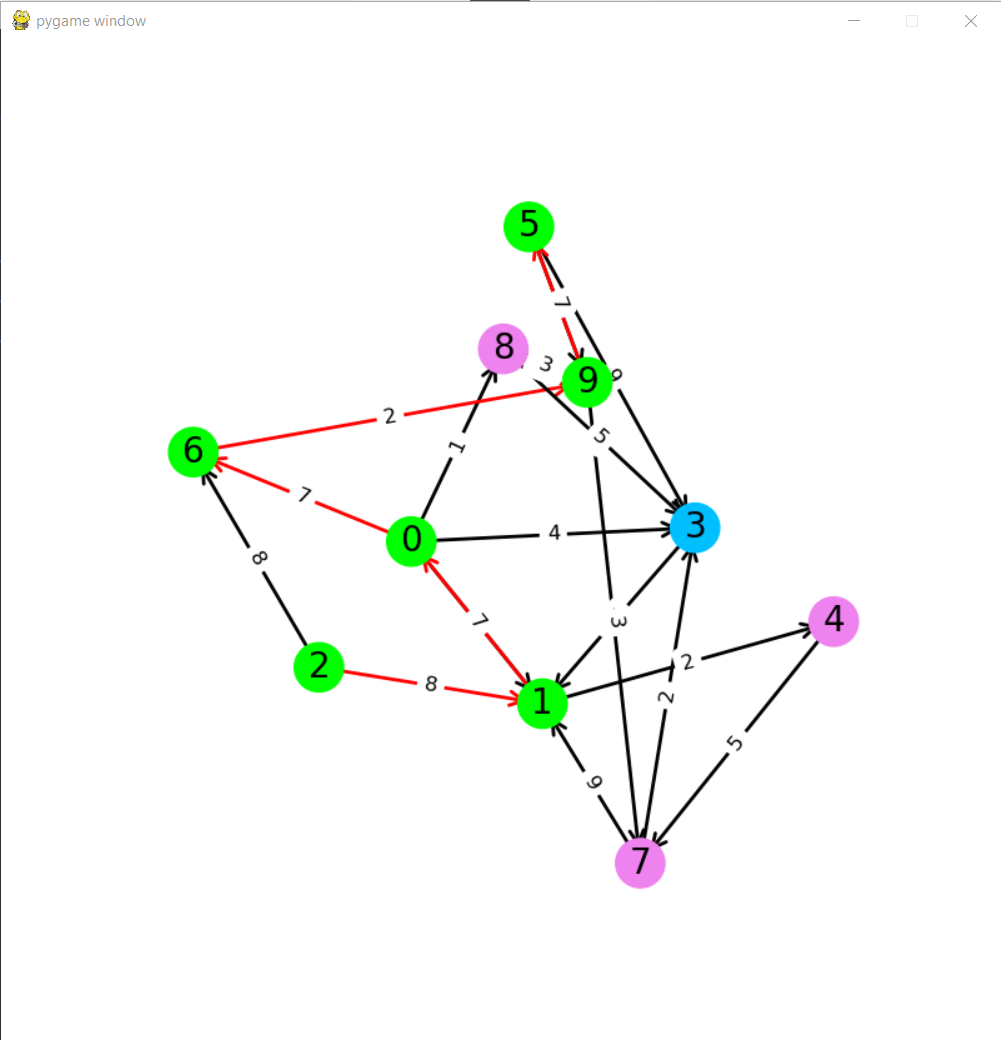
\includegraphics[width=0.5\textwidth]{result/testcase1/dfs.png}
    \caption{DFS}
\end{figure}
\begin{figure}[h!]
    \centering
    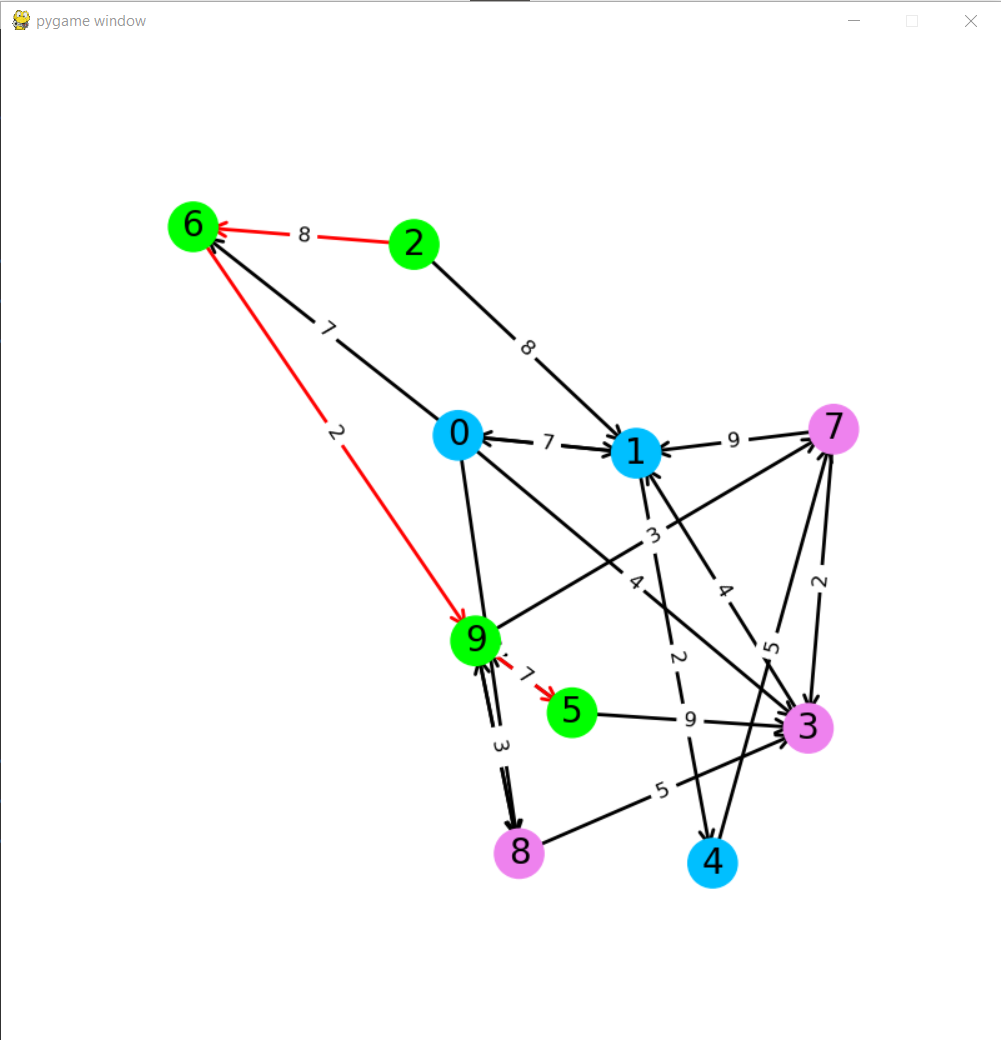
\includegraphics[width=0.5\textwidth]{result/testcase1/bfs.png}
    \caption{BFS}
\end{figure}
\begin{figure}[h!]
    \centering
    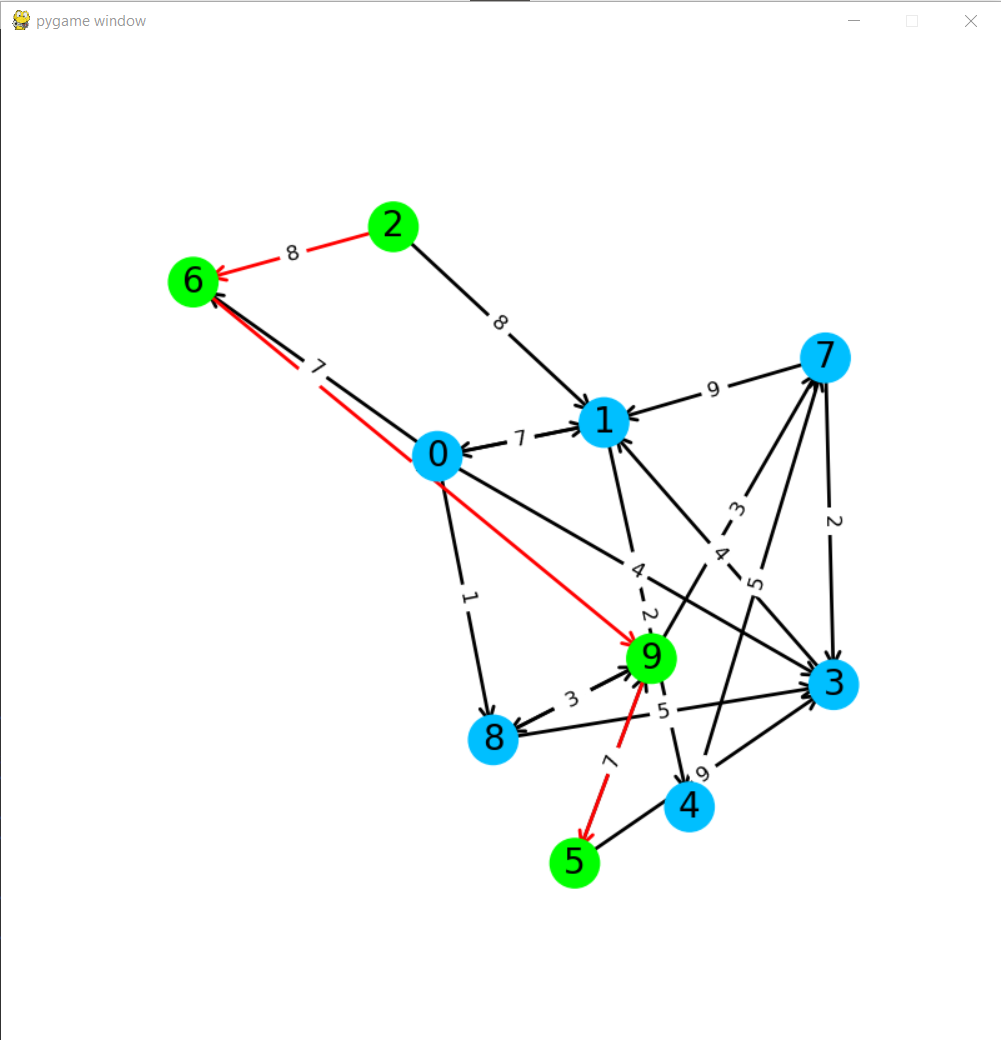
\includegraphics[width=0.5\textwidth]{result/testcase1/ucs.png}
    \caption{UCS}  
\end{figure}
\begin{figure}[h!]
    \centering
    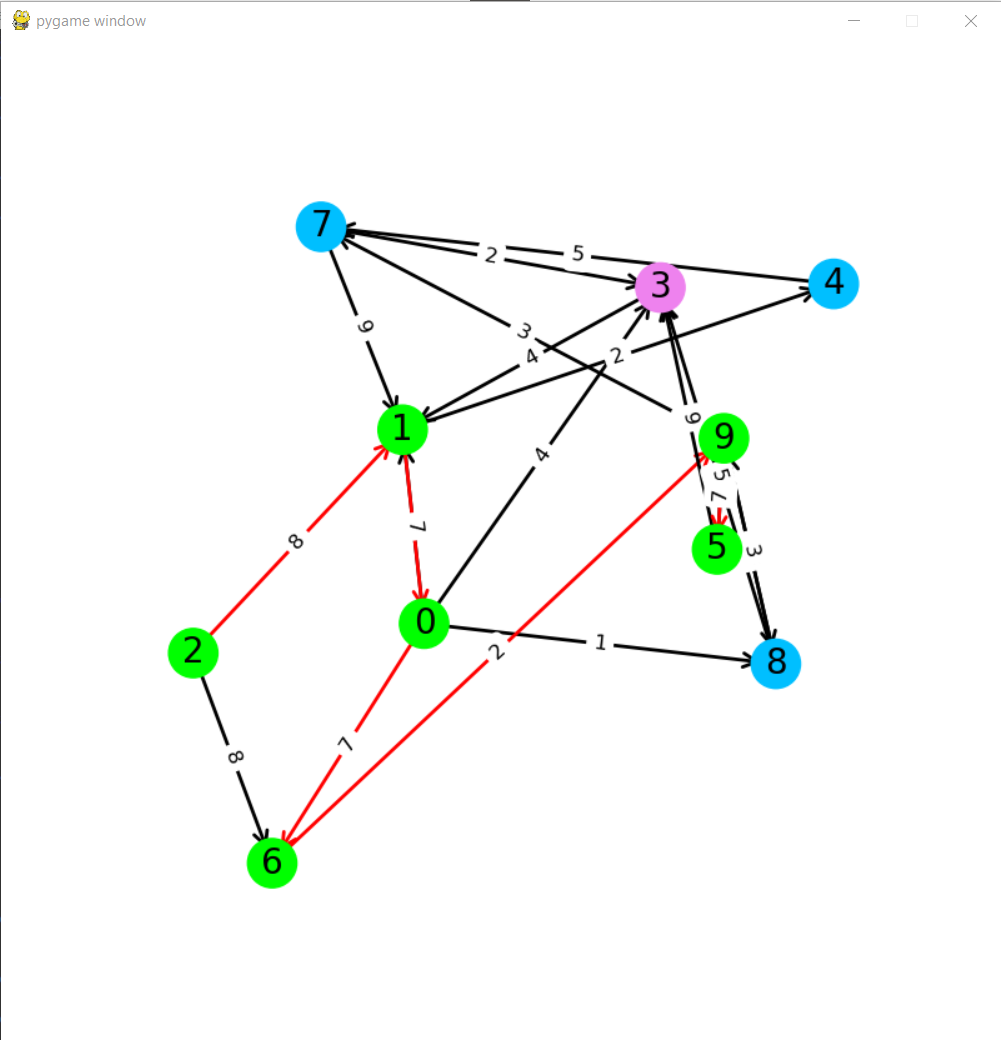
\includegraphics[width=0.5\textwidth]{result/testcase1/greedy.png}
    \caption{GBFS}
\end{figure}
\begin{figure}[h!]
    \centering
    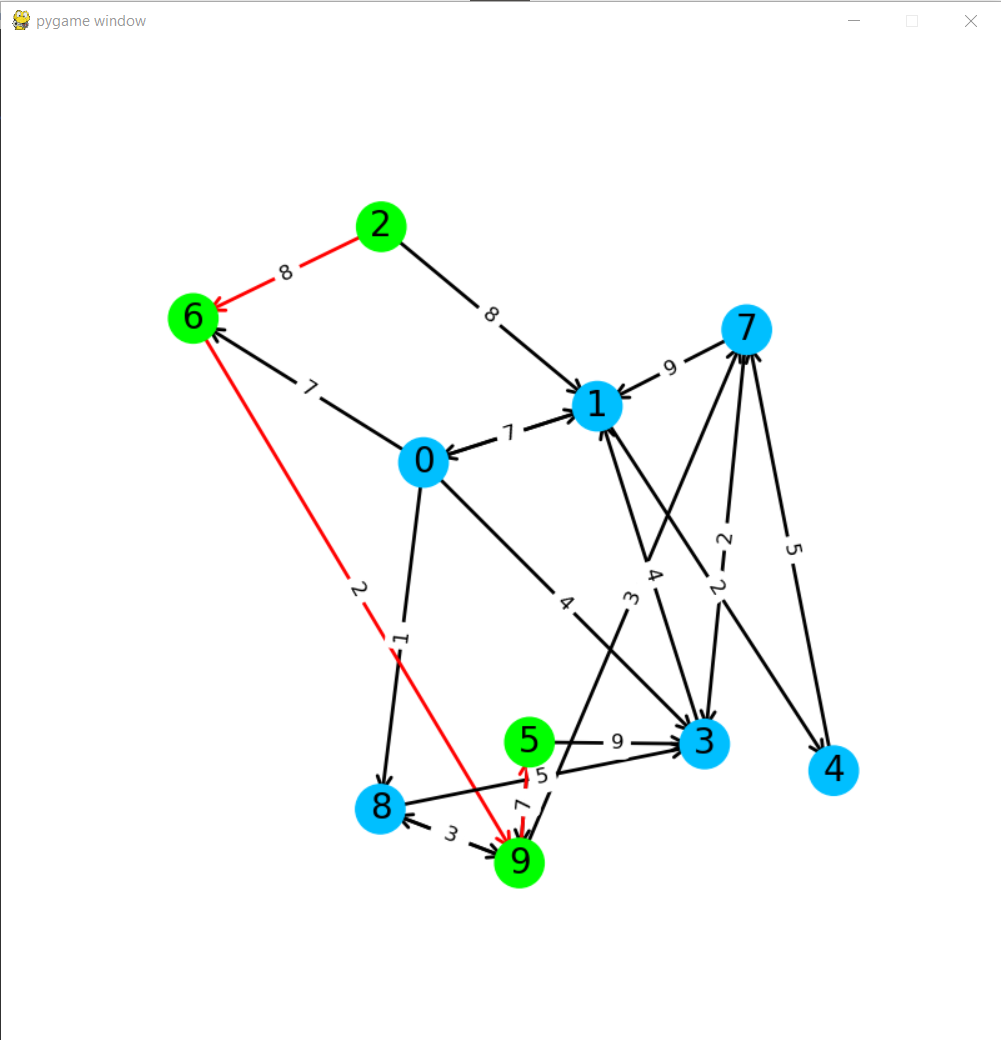
\includegraphics[width=0.5\textwidth]{result/testcase1/astar.png}
    \caption{A* with Euclidean Distance}
\end{figure}
\begin{figure}[h!]
    \centering
    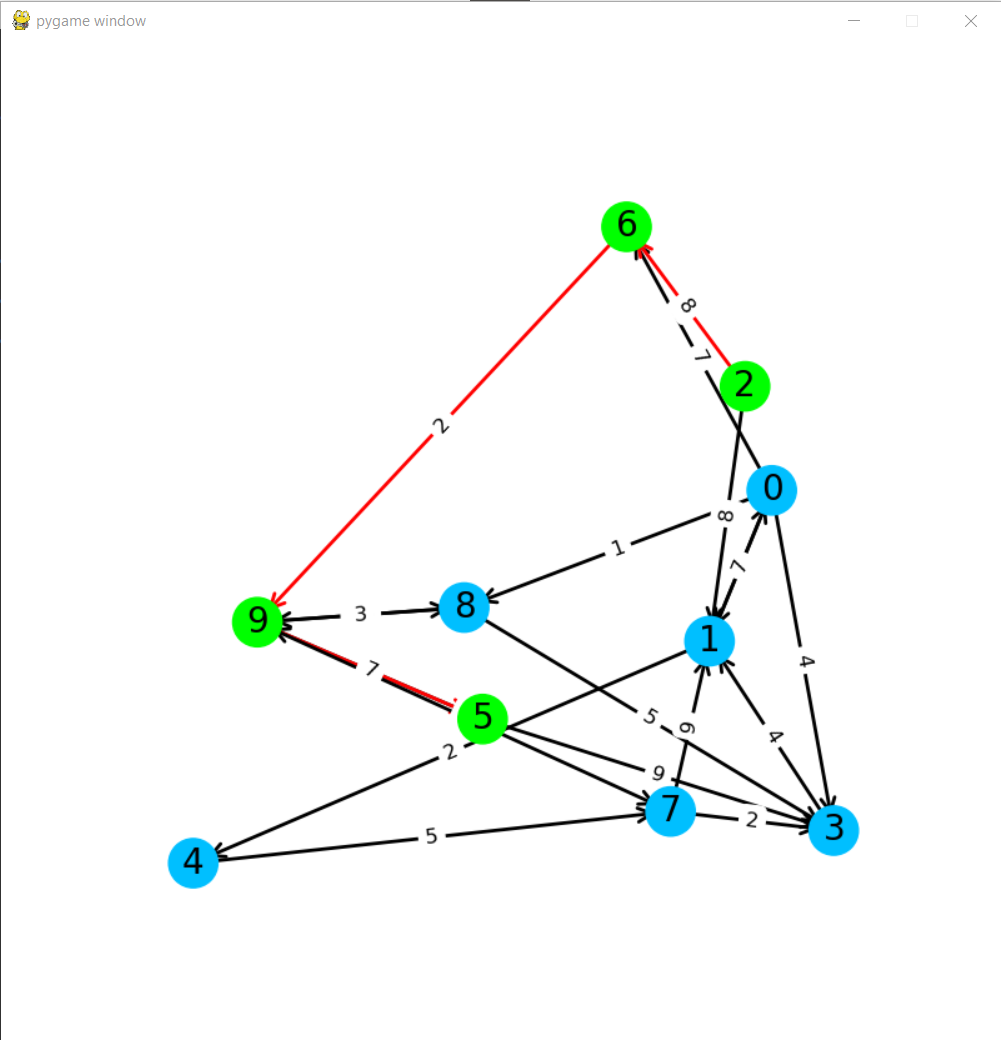
\includegraphics[width=0.5\textwidth]{result/testcase1/ids.png}
    \caption{IDS}
\end{figure}
\begin{figure}[h!]
    \centering
    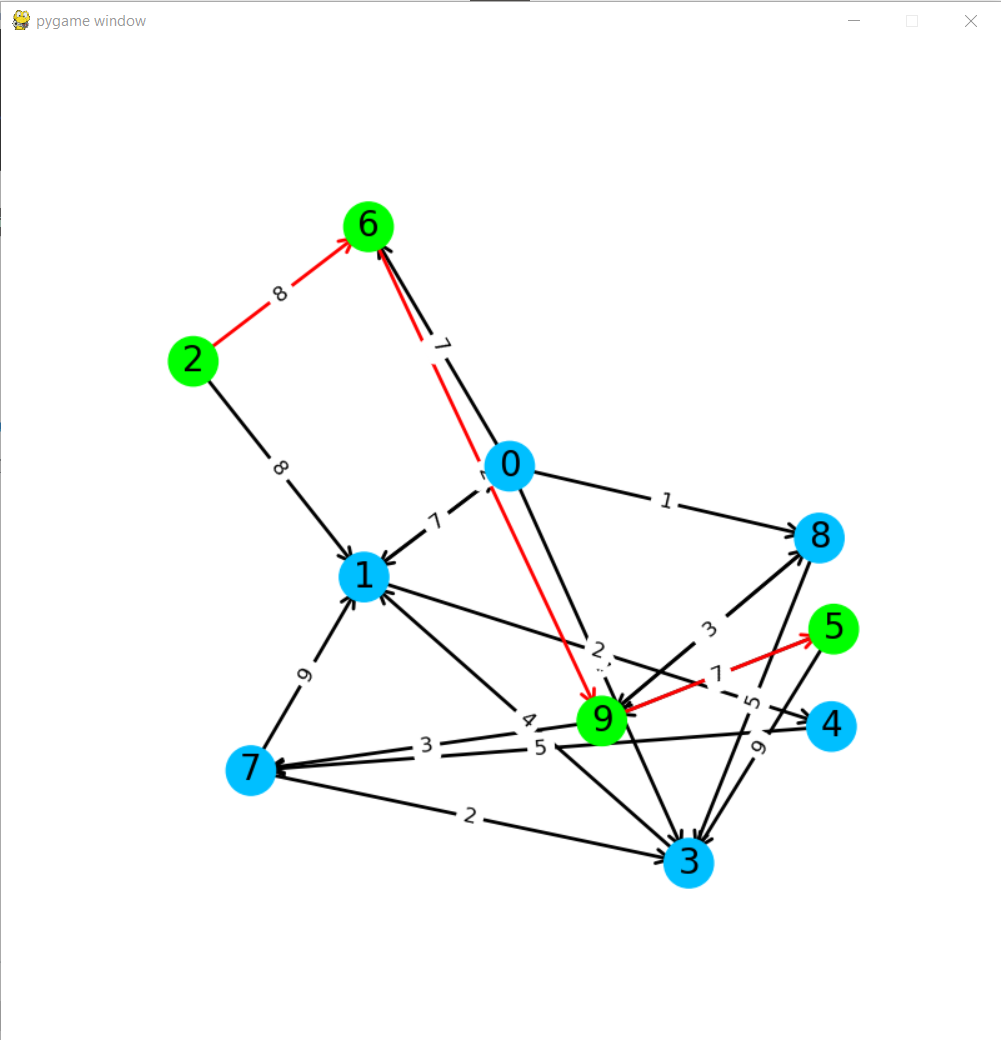
\includegraphics[width=0.5\textwidth]{result/testcase1/astar_2.png}
    \caption{A* with Manhattan Distance}
\end{figure}
\clearpage

\subsubsection{test case 2}
\begin{figure}[h!]
    \centering
    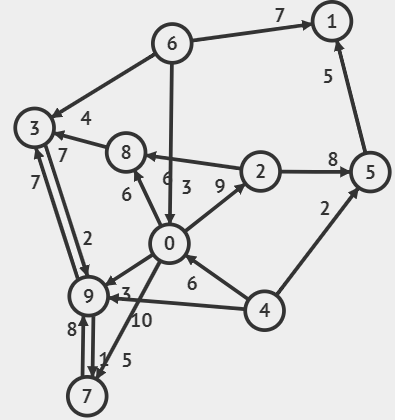
\includegraphics[width=0.5\textwidth]{testcase/2.PNG}
    \caption{Test Case 2 Image}
\end{figure}
\textbf{This is adjacency matrix for test case 2.} 
\begin{verbatim}
4 7
0 0 9 0 0 0 0 5 6 3
0 0 0 0 0 0 0 0 0 0
0 0 0 0 0 8 0 0 6 0
0 0 0 0 0 0 0 0 0 2
6 0 0 0 0 2 0 0 0 10
0 5 0 0 0 0 0 0 0 0
3 7 0 4 0 0 0 0 0 0
0 0 0 0 0 0 0 0 0 8
0 0 0 7 0 0 0 0 0 0
0 0 0 7 0 0 0 1 0 0
\end{verbatim}
\textbf{Test case Description:} 
\begin{itemize}
    \item Number of nodes: 10
    \item Number of edges: 20
    \item Start node: 4
    \item Goal node: 7
\end{itemize}

\paragraph*{Algorithm Results}
\quad The following are the results of the algorithms for test case 2.

\begin{figure}[h!]
    \centering
    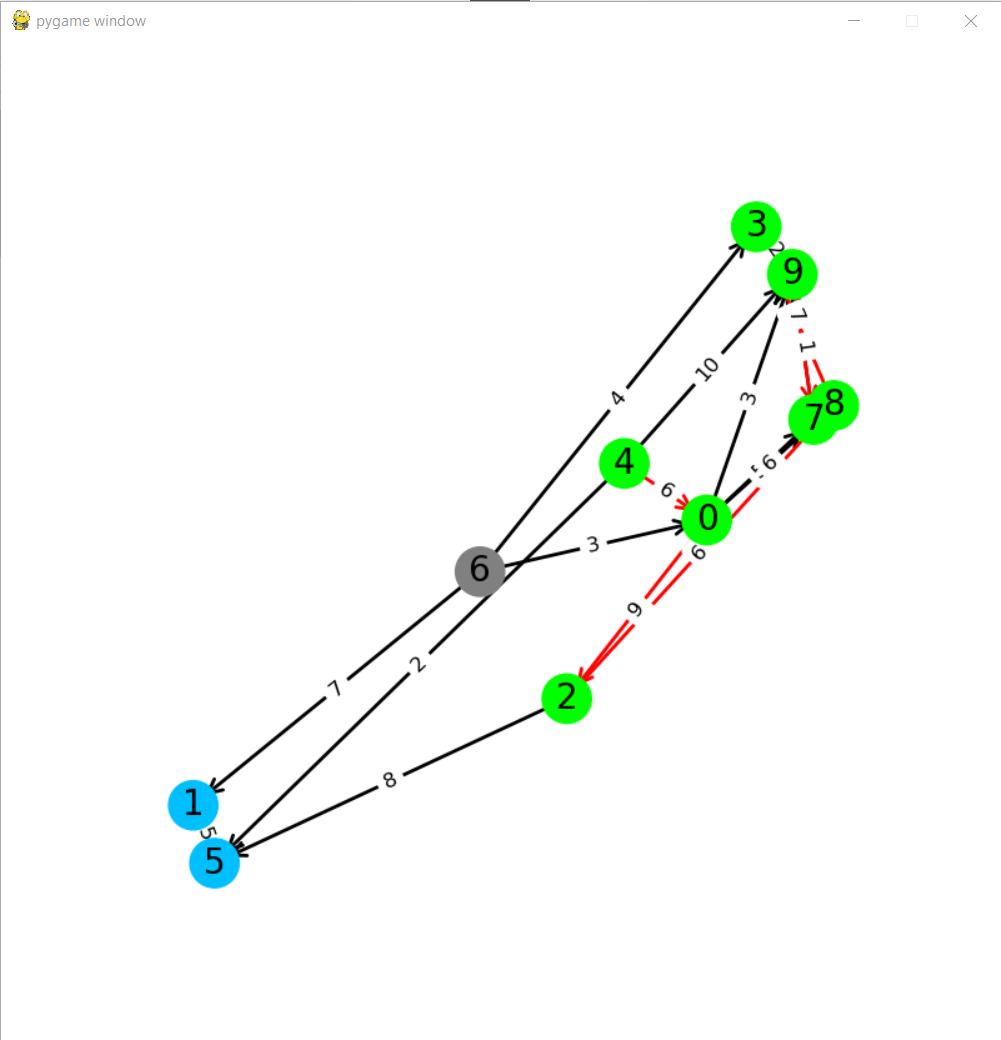
\includegraphics[width=0.5\textwidth]{result/testcase2/dfs.png}
    \caption{DFS}
\end{figure}
\begin{figure}[h!]
    \centering
    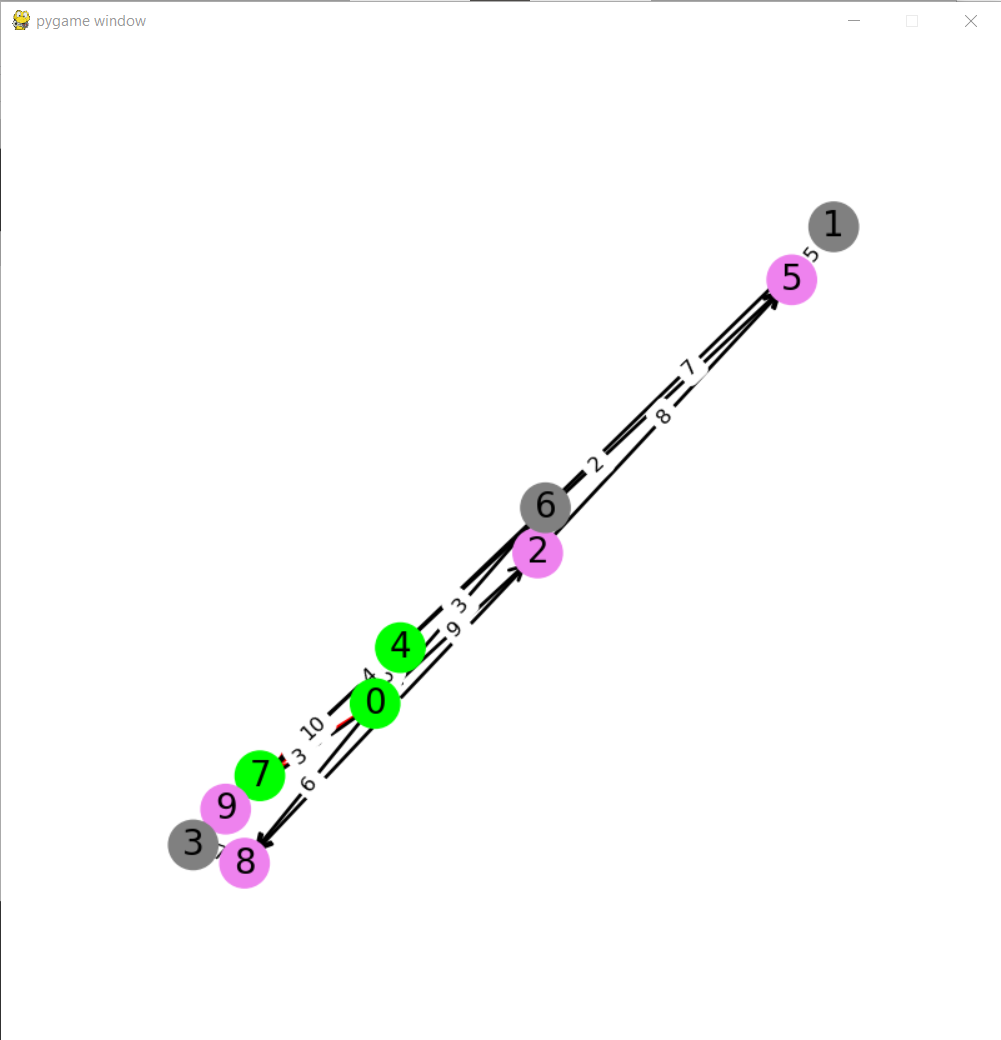
\includegraphics[width=0.5\textwidth]{result/testcase2/bfs.png}
    \caption{BFS}
\end{figure}
\begin{figure}[h!]
    \centering
    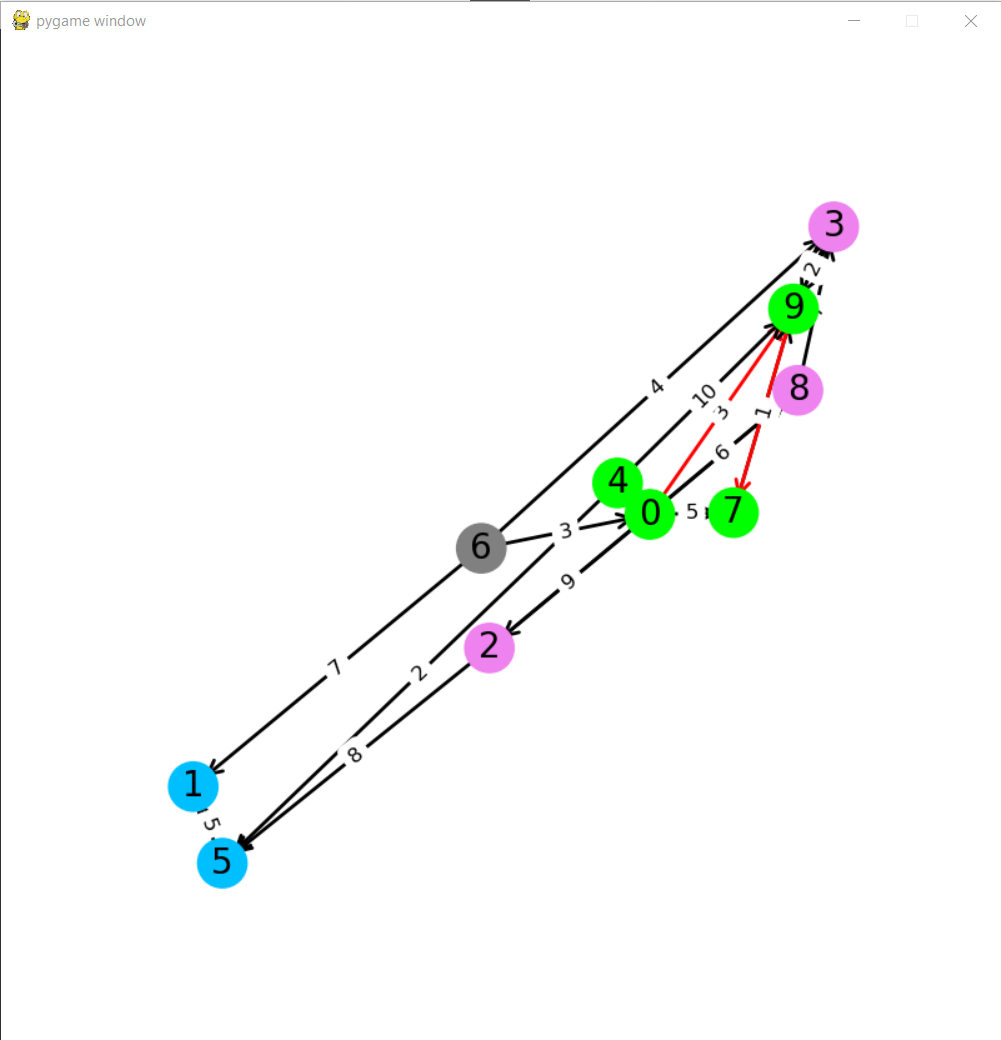
\includegraphics[width=0.5\textwidth]{result/testcase2/ucs.png}
    \caption{UCS}  
\end{figure}
\begin{figure}[h!]
    \centering
    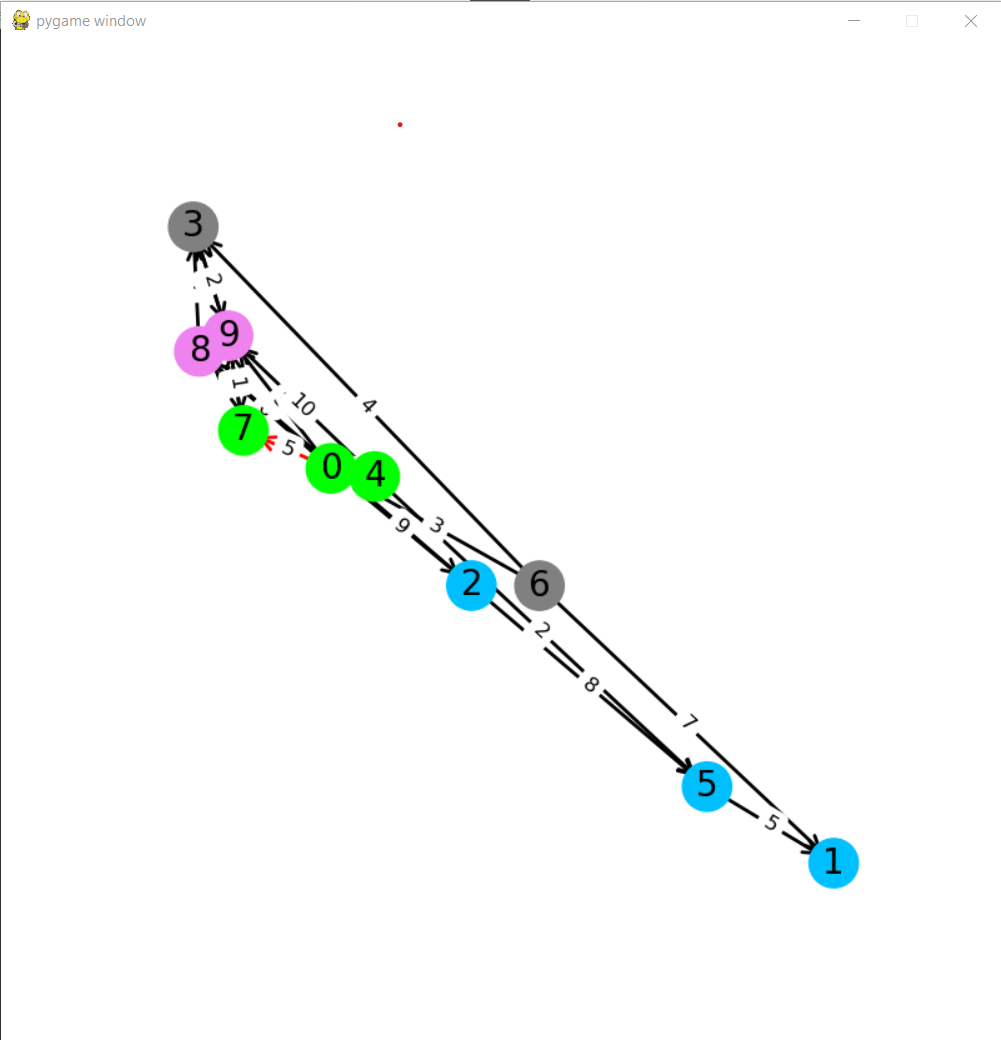
\includegraphics[width=0.5\textwidth]{result/testcase2/greedy.png}
    \caption{GBFS}
\end{figure}
\begin{figure}[h!]
    \centering
    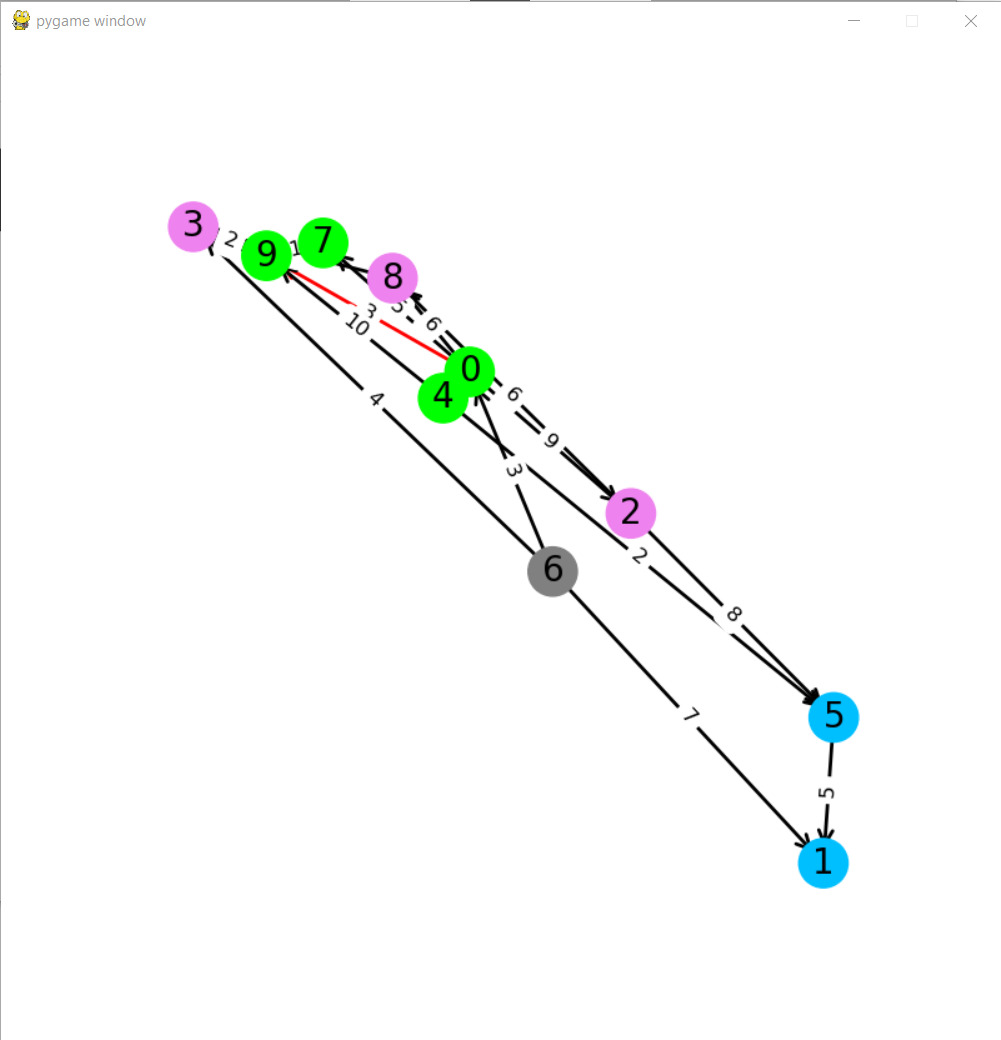
\includegraphics[width=0.5\textwidth]{result/testcase2/astar.png}
    \caption{A* with Euclidean Distance}
\end{figure}
\begin{figure}[h!]
    \centering
    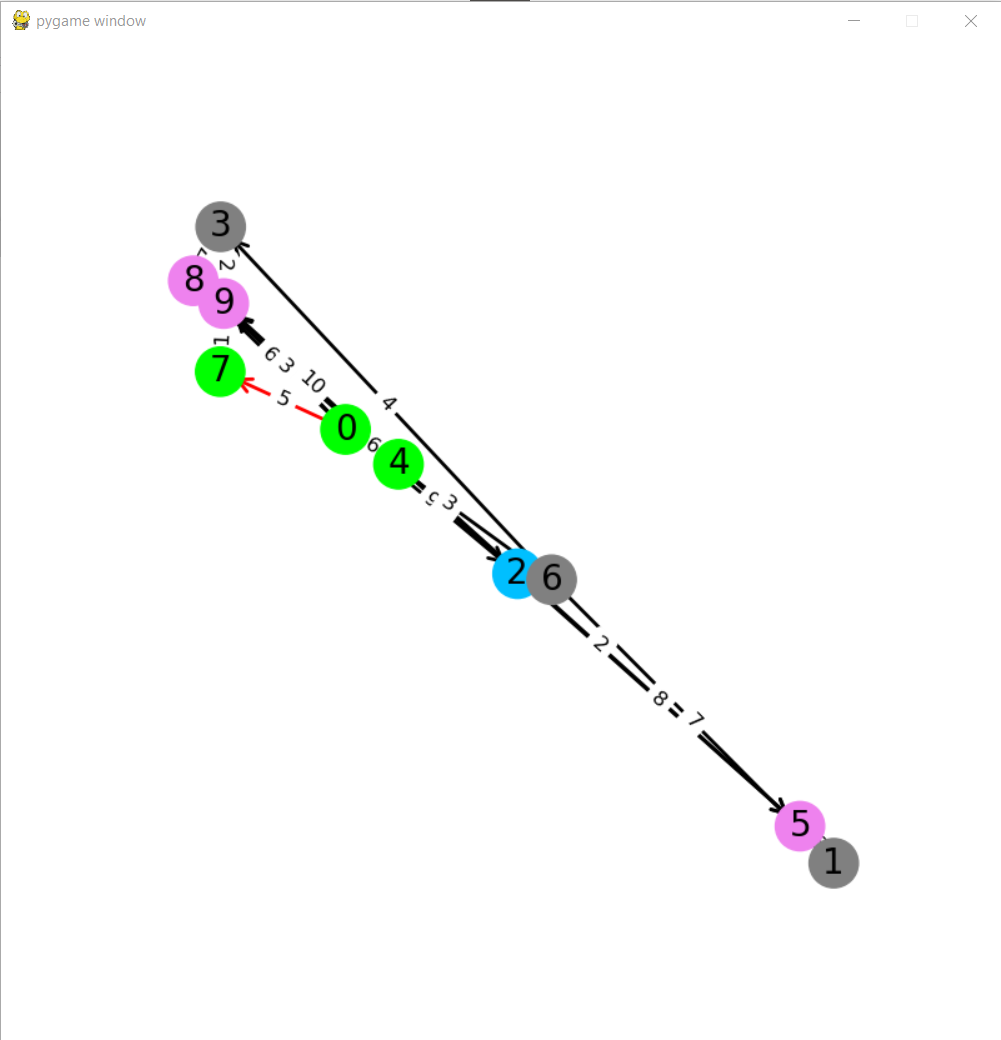
\includegraphics[width=0.5\textwidth]{result/testcase2/ids.png}
    \caption{IDS}
\end{figure}
\begin{figure}[h!]
    \centering
    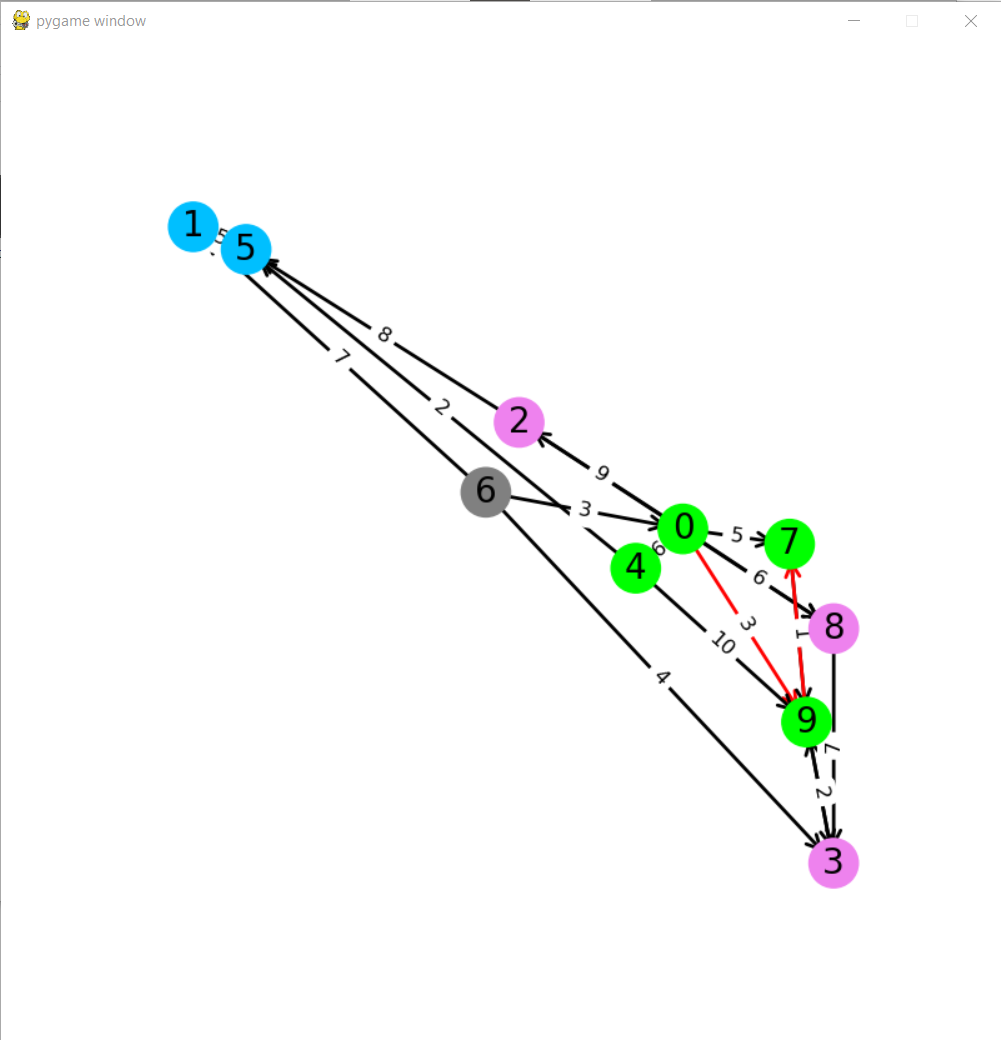
\includegraphics[width=0.5\textwidth]{result/testcase2/astar2.png}
    \caption{A* with Manhattan Distance}
\end{figure}
\clearpage
% continue for test case 3, 4, 5
\subsubsection{test case 3}
\begin{figure}[h!]
    \centering
    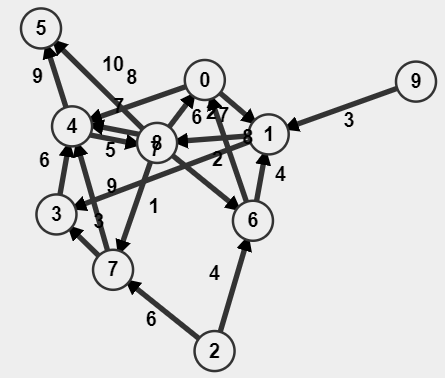
\includegraphics[width=0.5\textwidth]{testcase/3.PNG}
    \caption{Test Case 3 Image}
\end{figure}
\textbf{This is adjacency matrix for test case 3.}
\begin{verbatim}
2 5
0 7 0 0 8 0 0 0 0 0
0 0 0 7 0 0 0 0 2 0
0 0 0 0 0 0 4 6 0 0
0 0 0 0 6 0 0 0 0 0
0 0 0 0 0 9 0 0 5 0
0 0 0 0 0 0 0 0 0 0
8 4 0 0 0 0 0 0 0 0
0 0 0 3 9 0 0 0 0 0
6 0 0 0 7 10 2 1 0 0
0 3 0 0 0 0 0 0 0 0    
\end{verbatim}
\textbf{Test case Description:}
\begin{itemize}
    \item Number of nodes: 10 
    \item Number of edges: 20
    \item Start node: 2
    \item Goal node: 5
\end{itemize}

\paragraph*{Algorithm Results}

\quad The following are the results of the algorithms for test case 3.

\begin{figure}[h!]
    \centering
    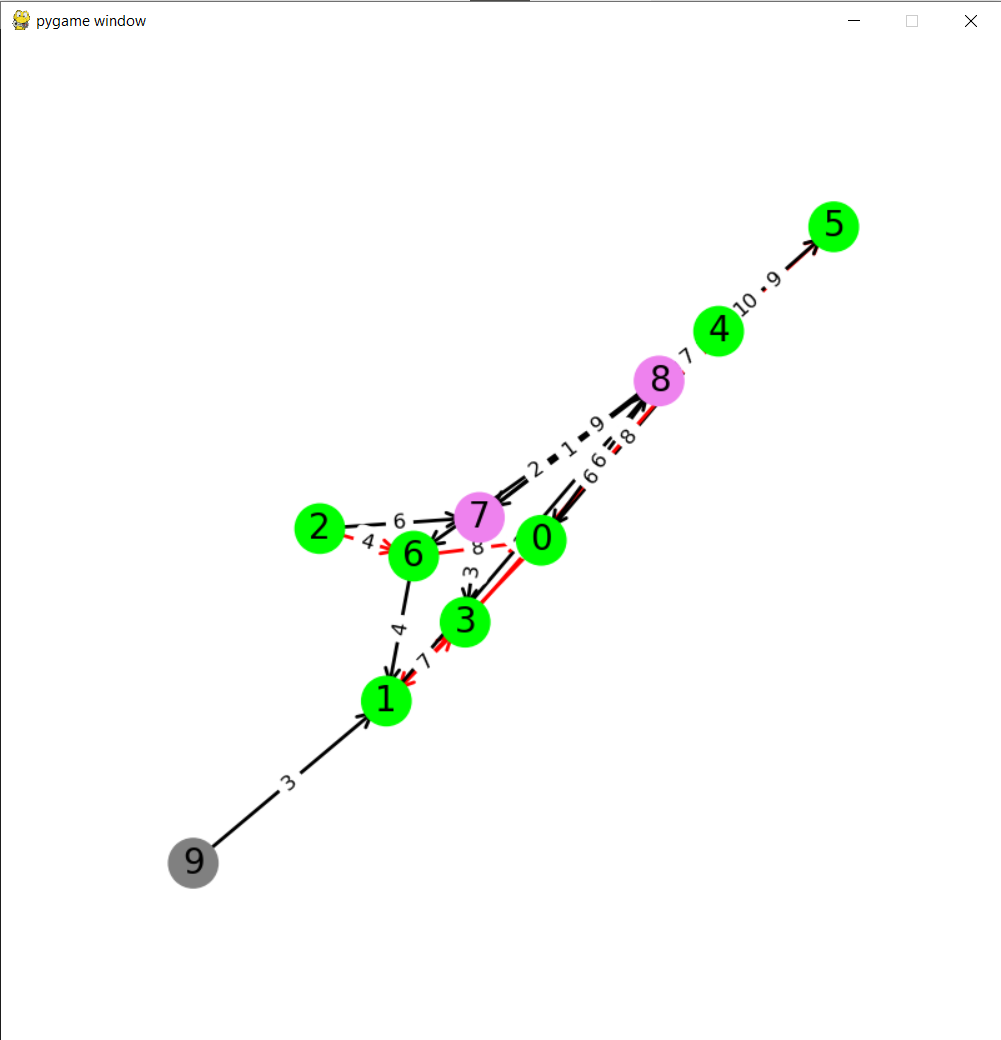
\includegraphics[width=0.5\textwidth]{result/testcase3/dfs.png}
    \caption{DFS}
\end{figure}
\begin{figure}[h!]
    \centering
    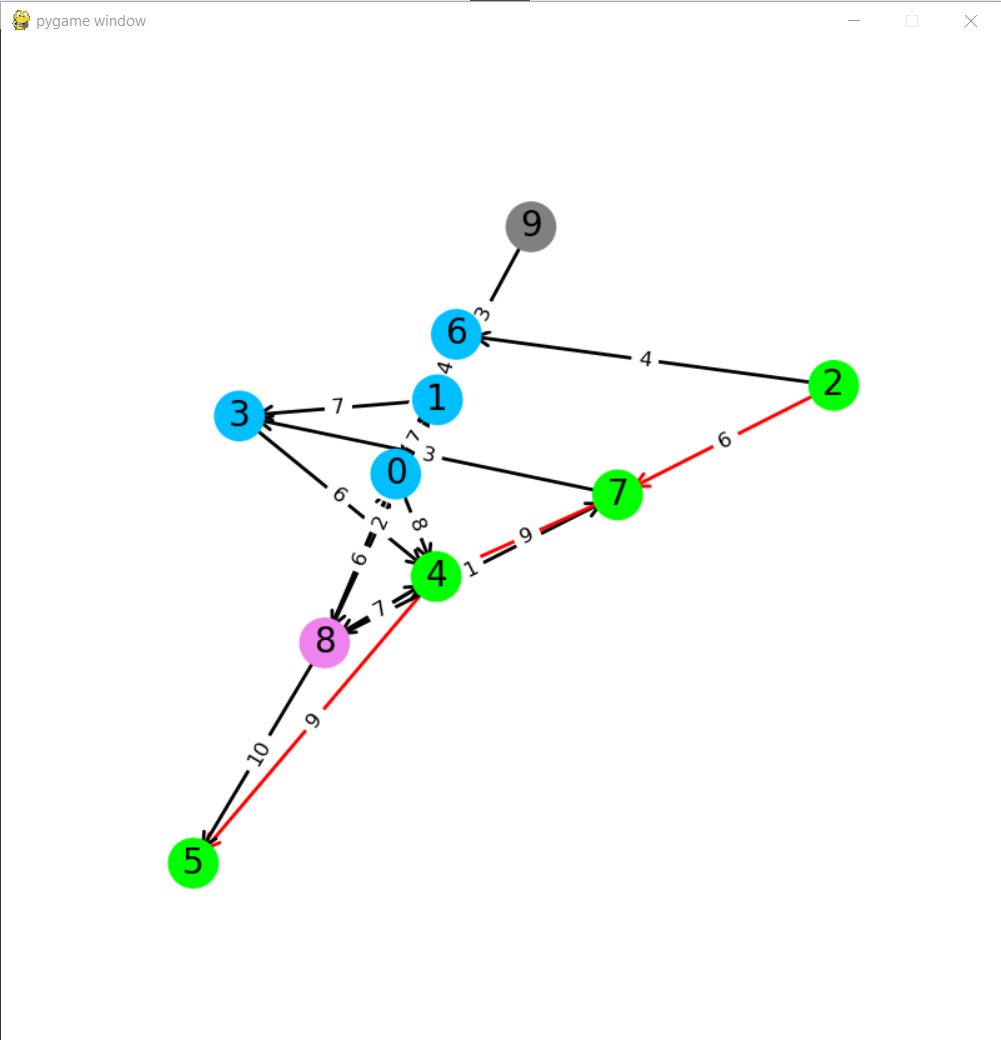
\includegraphics[width=0.5\textwidth]{result/testcase3/bfs.png}
    \caption{BFS}
\end{figure}
\begin{figure}[h!]
    \centering
    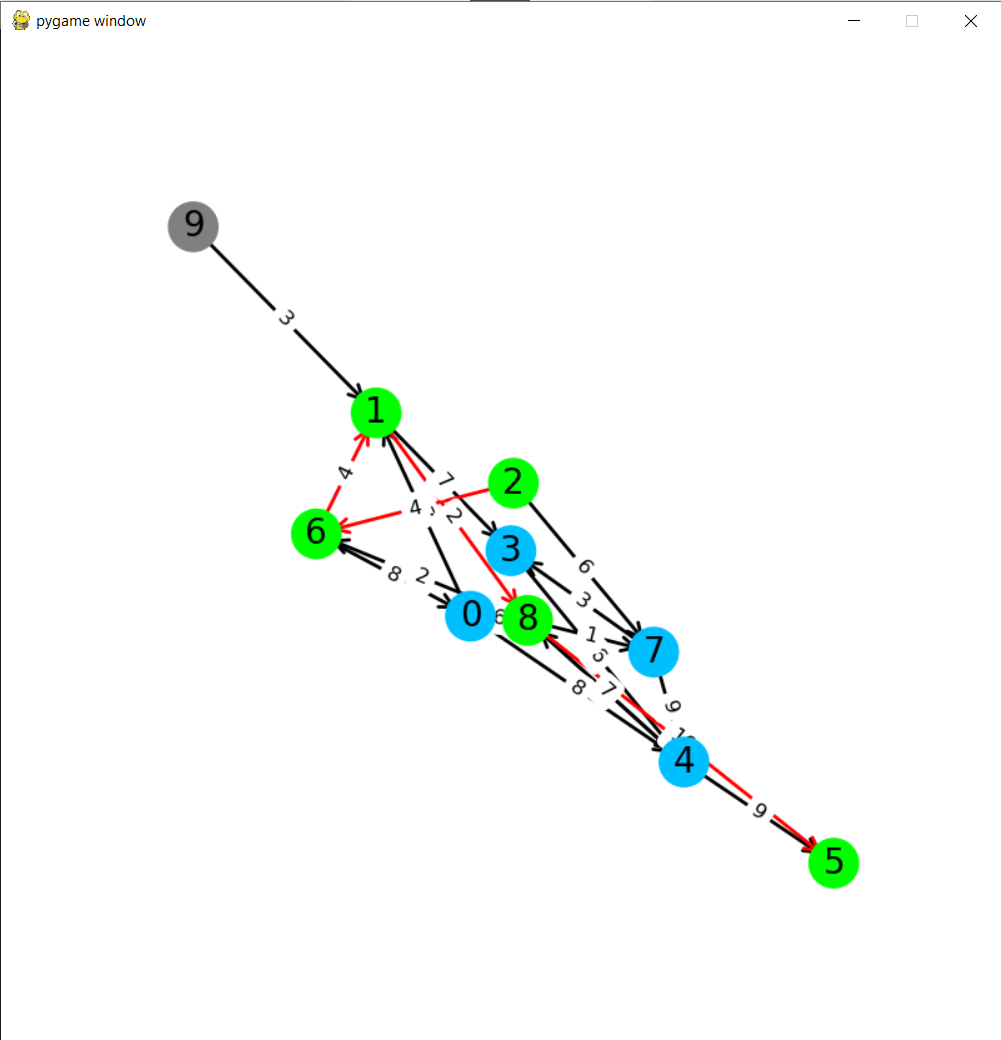
\includegraphics[width=0.5\textwidth]{result/testcase3/ucs.png}
    \caption{UCS}  
\end{figure}
\begin{figure}[h!]
    \centering
    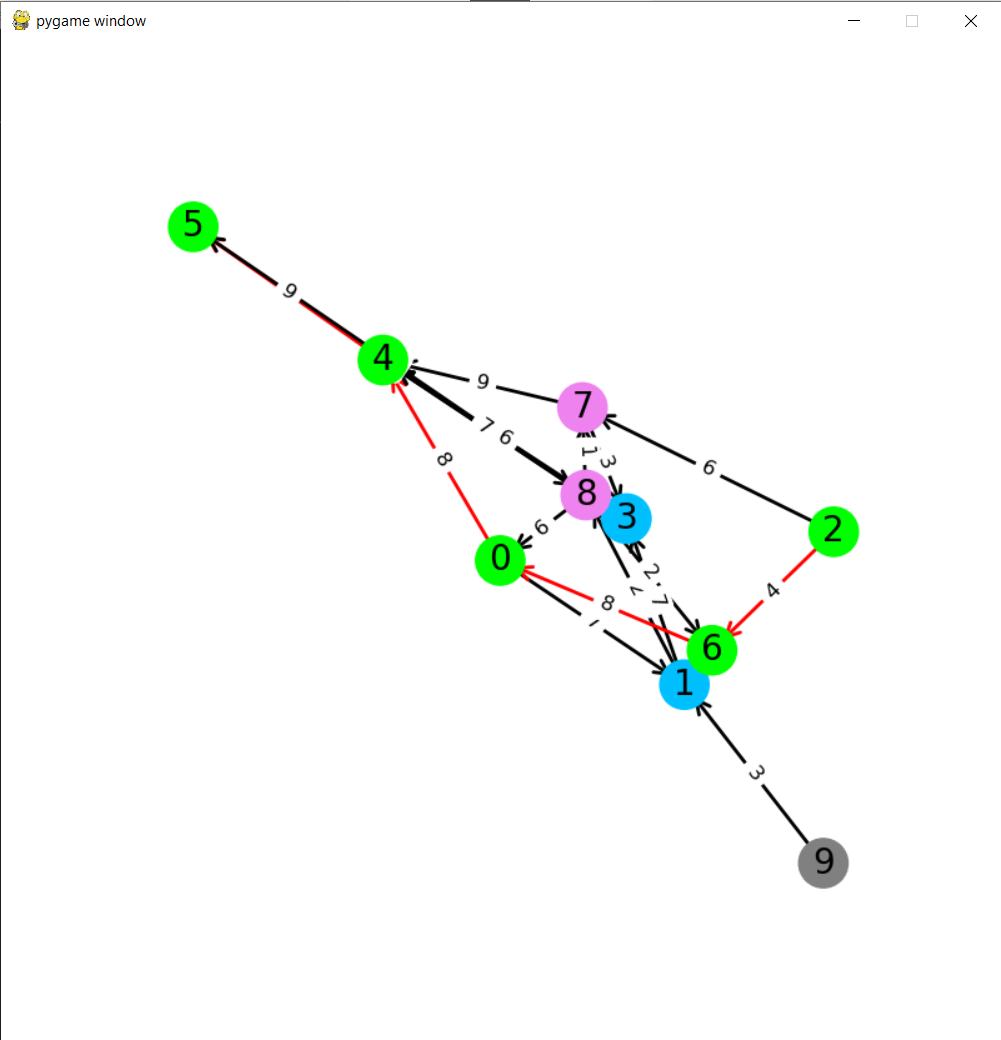
\includegraphics[width=0.5\textwidth]{result/testcase3/greedy.png}
    \caption{GBFS}
\end{figure}
\begin{figure}[h!]
    \centering
    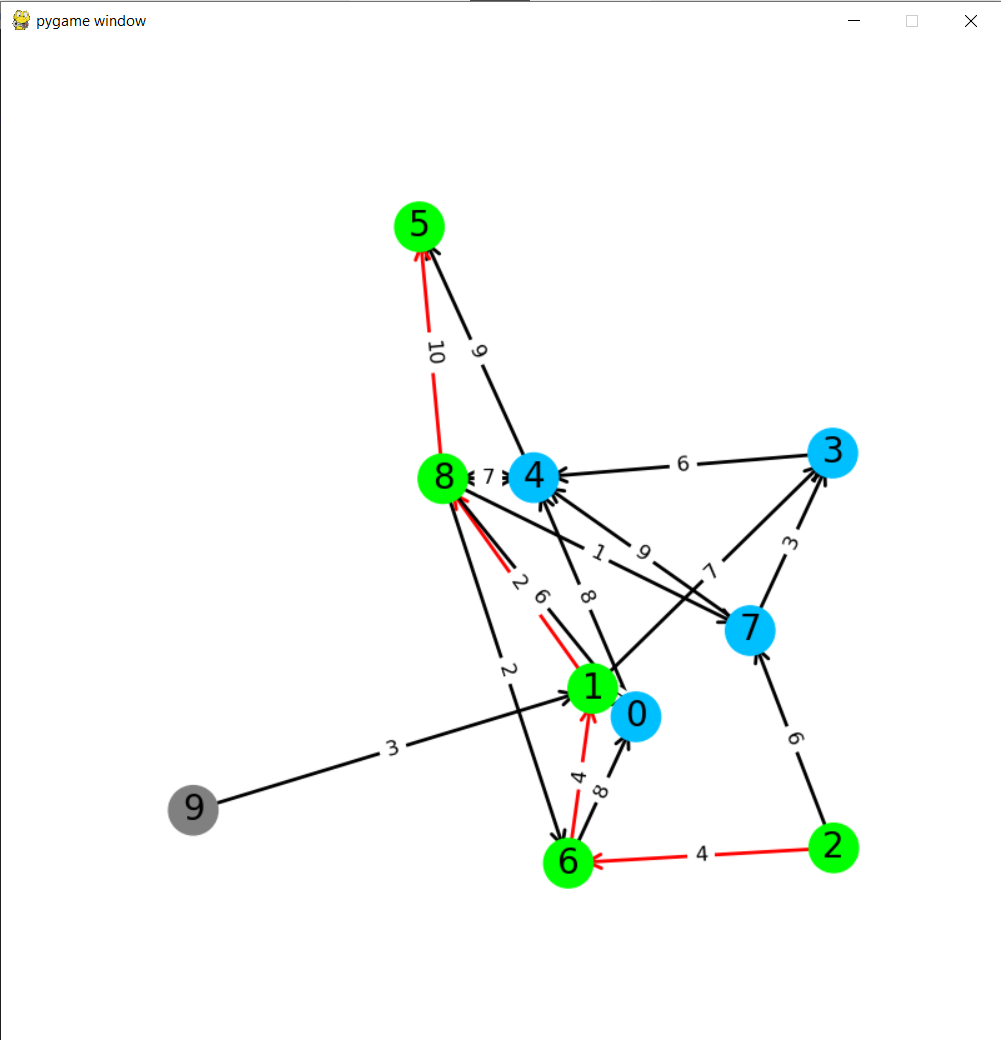
\includegraphics[width=0.5\textwidth]{result/testcase3/astar.png}
    \caption{A* with Euclidean Distance}
\end{figure}
\begin{figure}[h!]
    \centering
    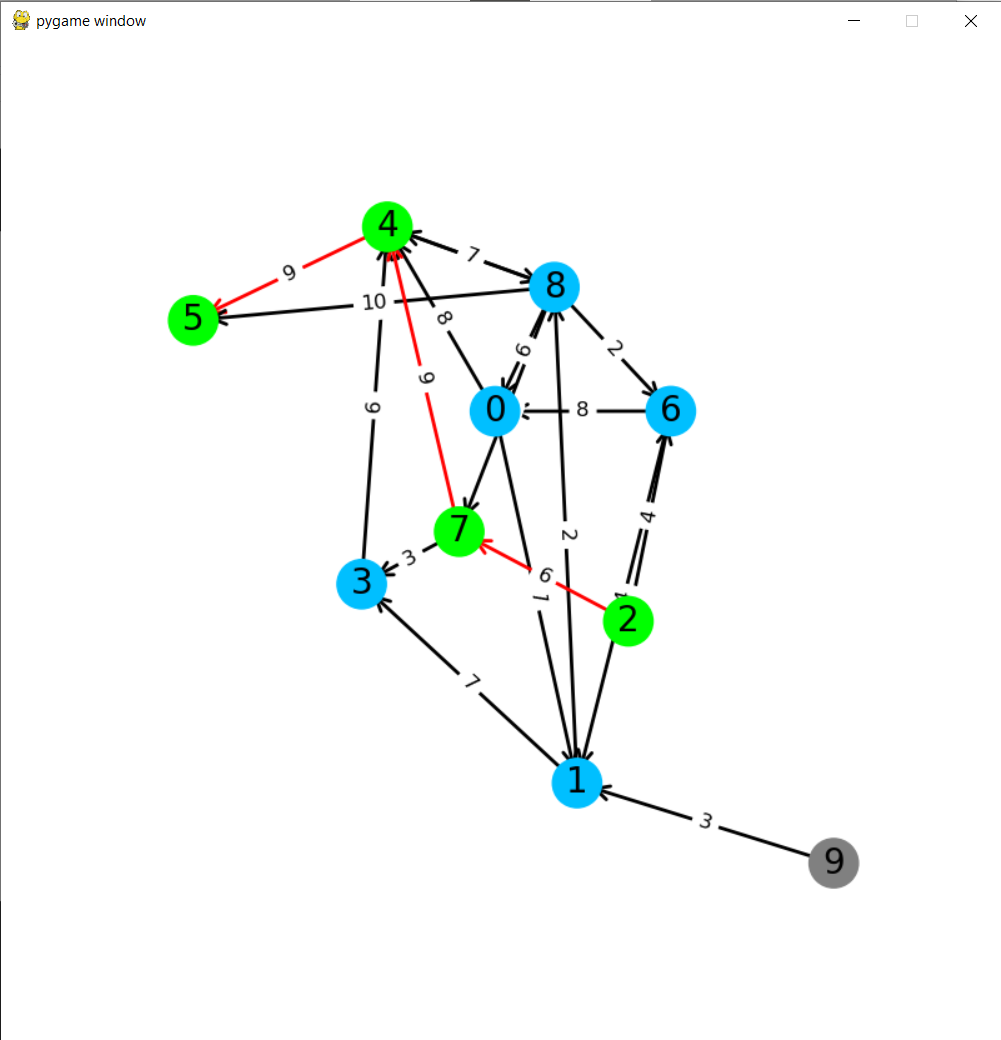
\includegraphics[width=0.5\textwidth]{result/testcase3/ids.png}
    \caption{IDS}
\end{figure}
\begin{figure}[h!]
    \centering
    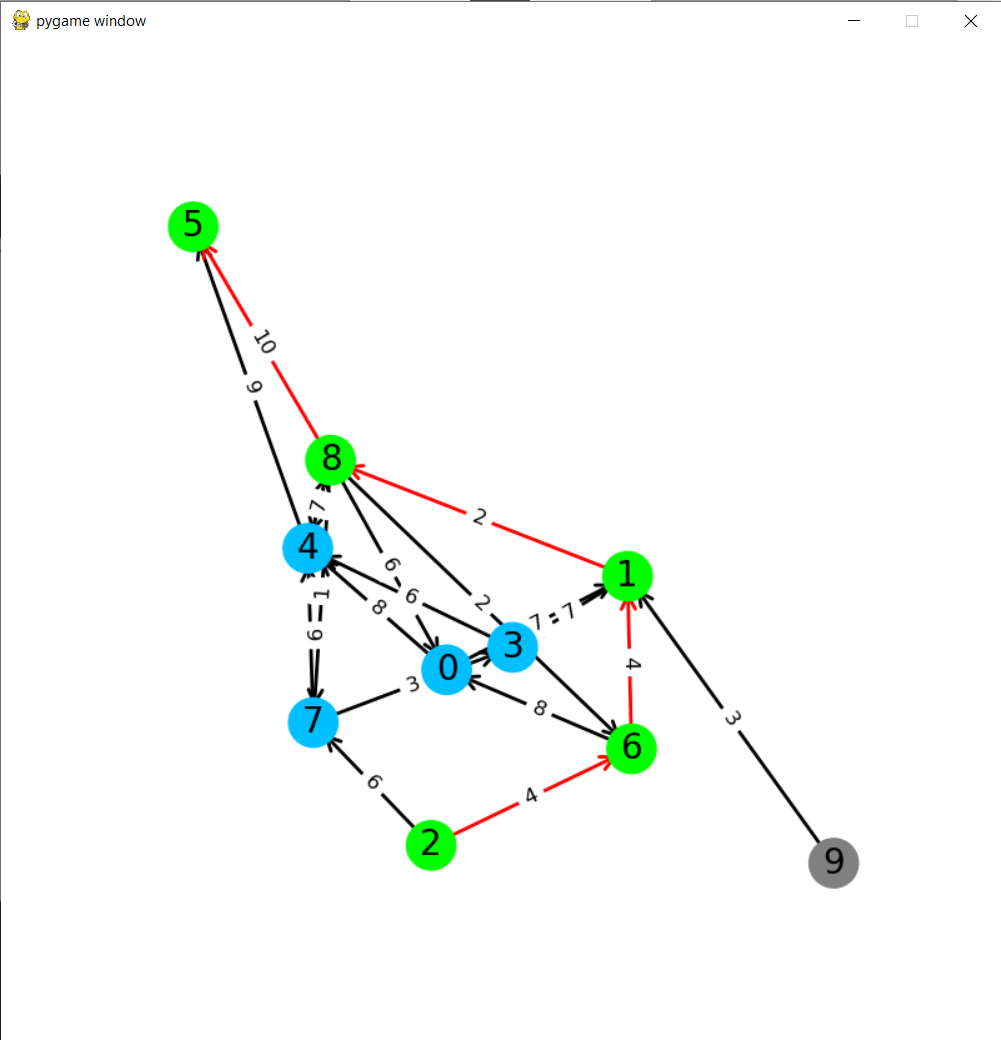
\includegraphics[width=0.5\textwidth]{result/testcase3/astar2.png}
    \caption{A* with Manhattan Distance}
\end{figure}
\clearpage 

\subsubsection{test case 4}
\begin{figure}[h!]
    \centering
    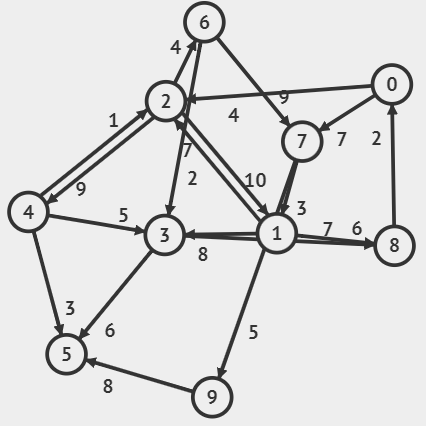
\includegraphics[width=0.5\textwidth]{testcase/4.PNG}
    \caption{Test Case 4 Image}
\end{figure}
\textbf{This is adjacency matrix for test case 4.}
\begin{verbatim}
0 5
0 0 4 0 0 0 0 7 0 0
0 0 7 8 0 0 0 0 6 0
0 10 0 0 9 0 4 0 0 0
0 0 0 0 0 6 0 0 7 0
0 0 1 5 0 3 0 0 0 0
0 0 0 0 0 0 0 0 0 0
0 0 0 2 0 0 0 9 0 0
0 3 0 0 0 0 0 0 0 5
2 0 0 0 0 0 0 0 0 0
0 0 0 0 0 8 0 0 0 0   
\end{verbatim}
\textbf{Test case Description:}
\begin{itemize}
    \item Number of nodes: 10 
    \item Number of edges: 20
    \item Start node: 0
    \item Goal node: 5
\end{itemize}

\paragraph*{Algorithm Results}

\quad The following are the results of the algorithms for test case 4.

\begin{figure}[h!]
    \centering
    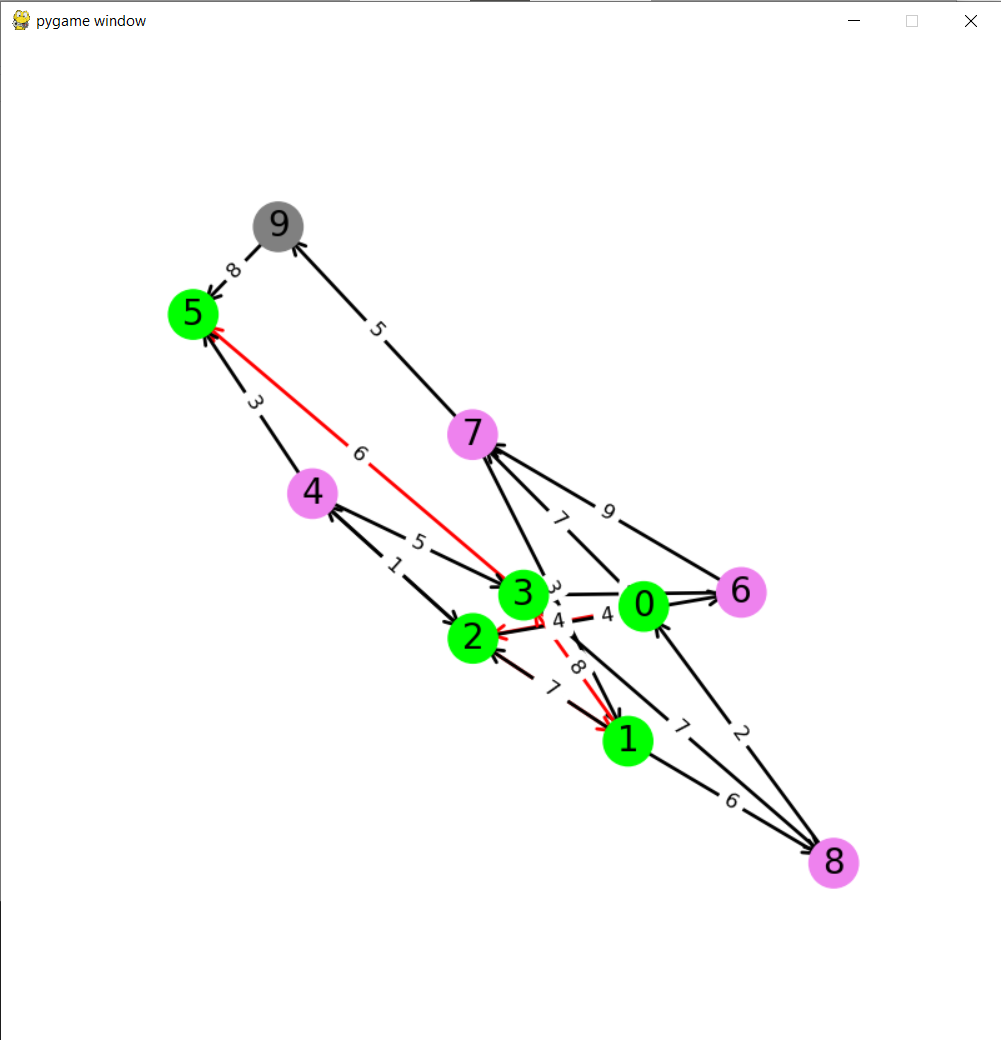
\includegraphics[width=0.5\textwidth]{result/testcase4/dfs.png}
    \caption{DFS}
\end{figure}
\begin{figure}[h!]
    \centering
    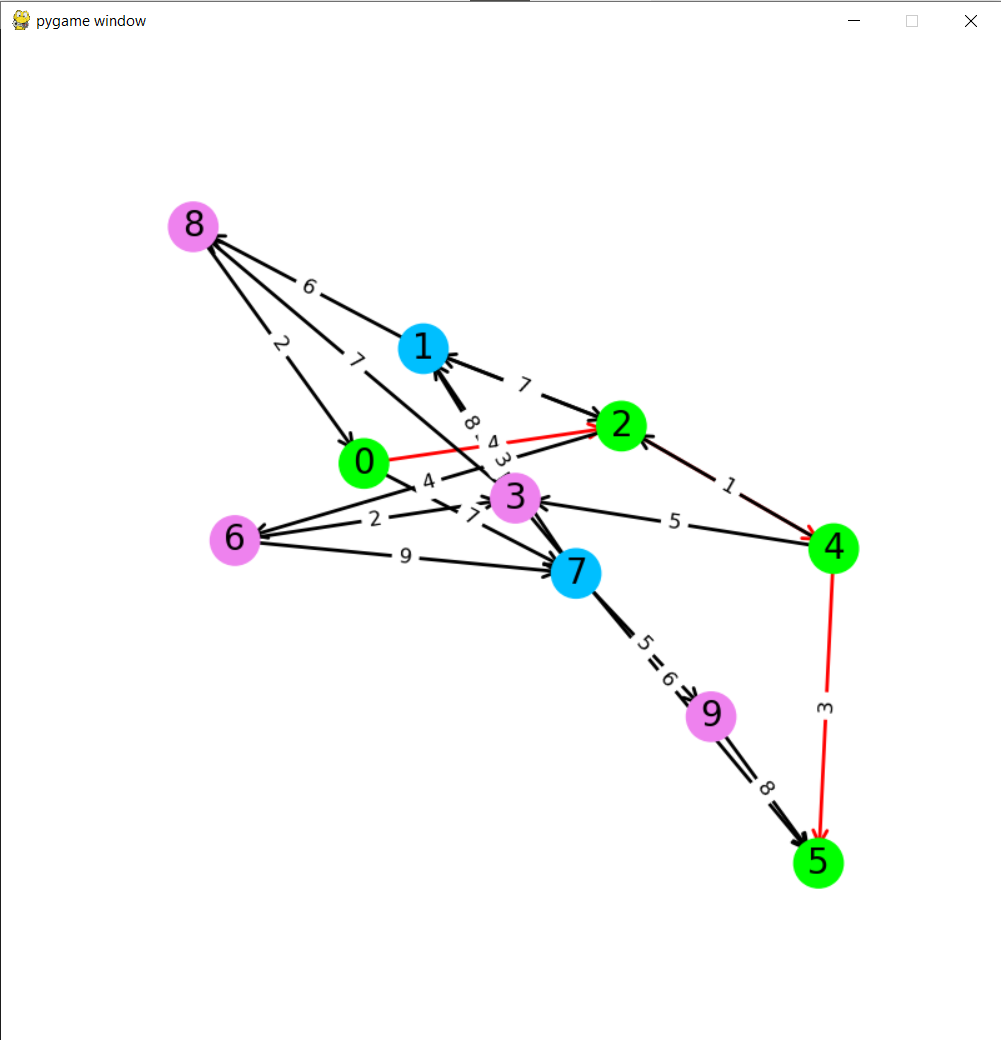
\includegraphics[width=0.5\textwidth]{result/testcase4/bfs.png}
    \caption{BFS}
\end{figure}
\begin{figure}[h!]
    \centering
    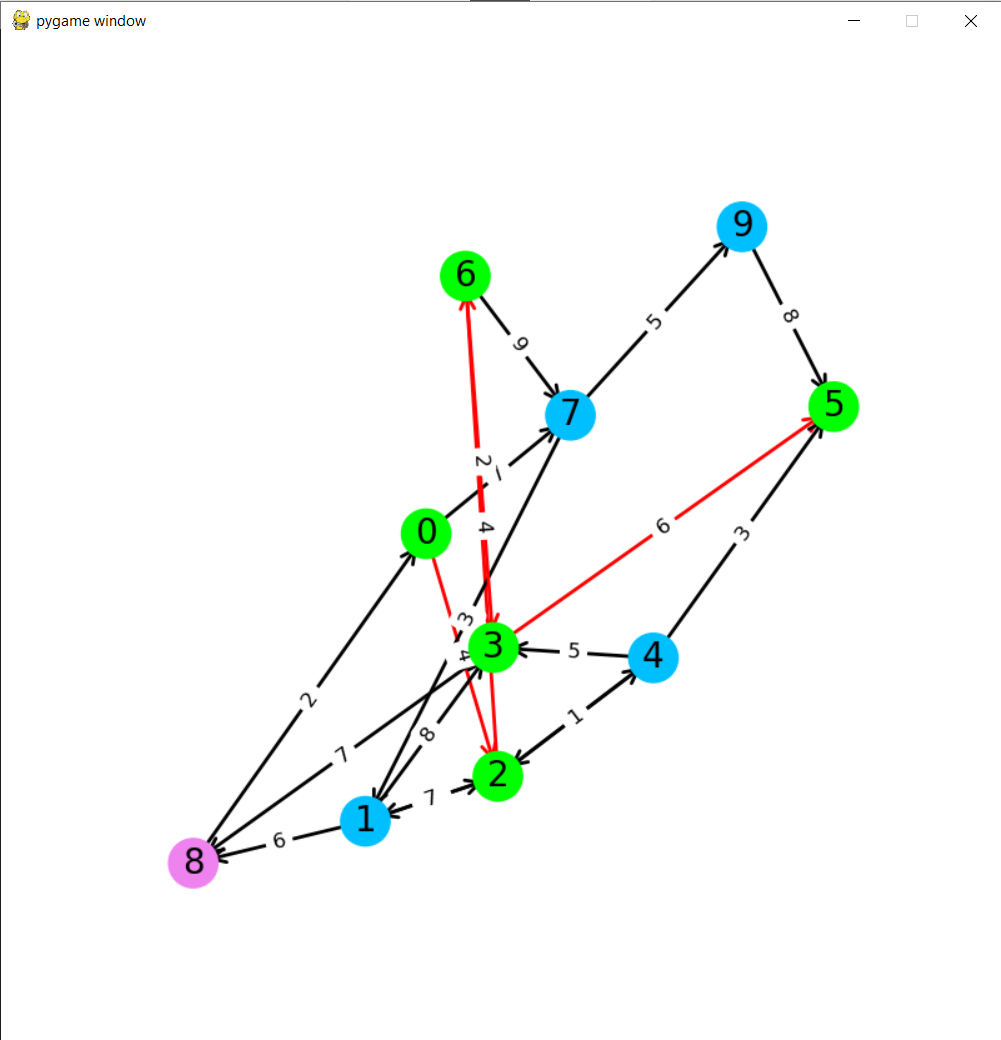
\includegraphics[width=0.5\textwidth]{result/testcase4/ucs.png}
    \caption{UCS}  
\end{figure}
\begin{figure}[h!]
    \centering
    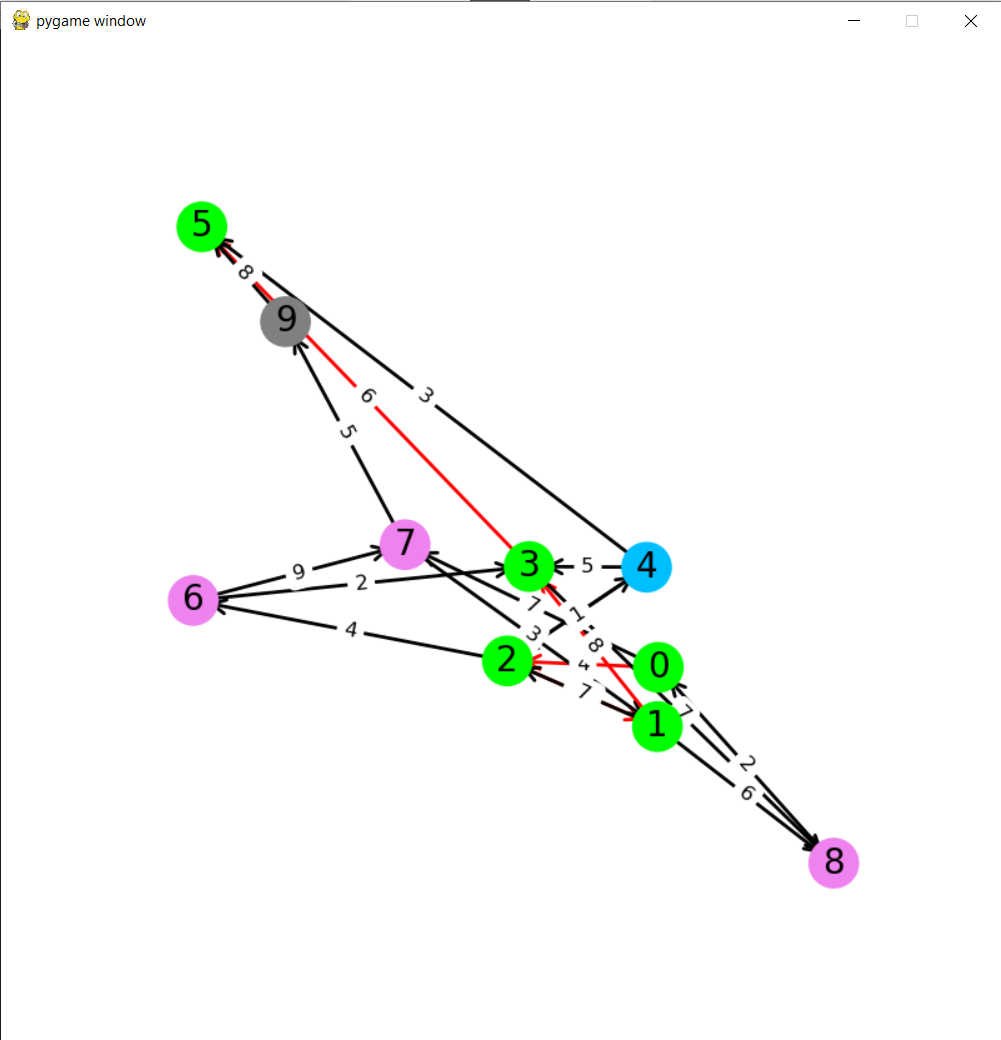
\includegraphics[width=0.5\textwidth]{result/testcase4/greedy.png}
    \caption{GBFS}
\end{figure}
\begin{figure}[h!]
    \centering
    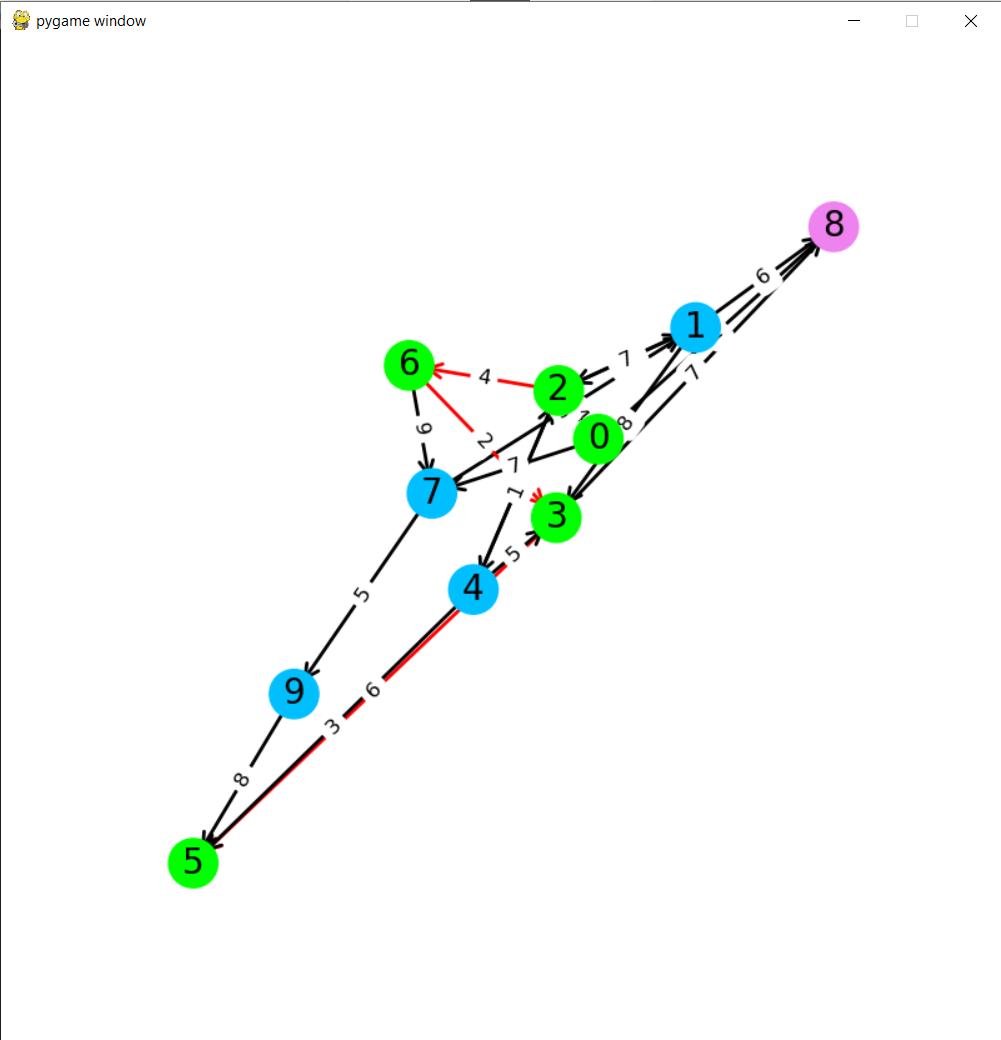
\includegraphics[width=0.5\textwidth]{result/testcase4/astar.png}
    \caption{A* with Euclidean Distance}
\end{figure}
\begin{figure}[h!]
    \centering
    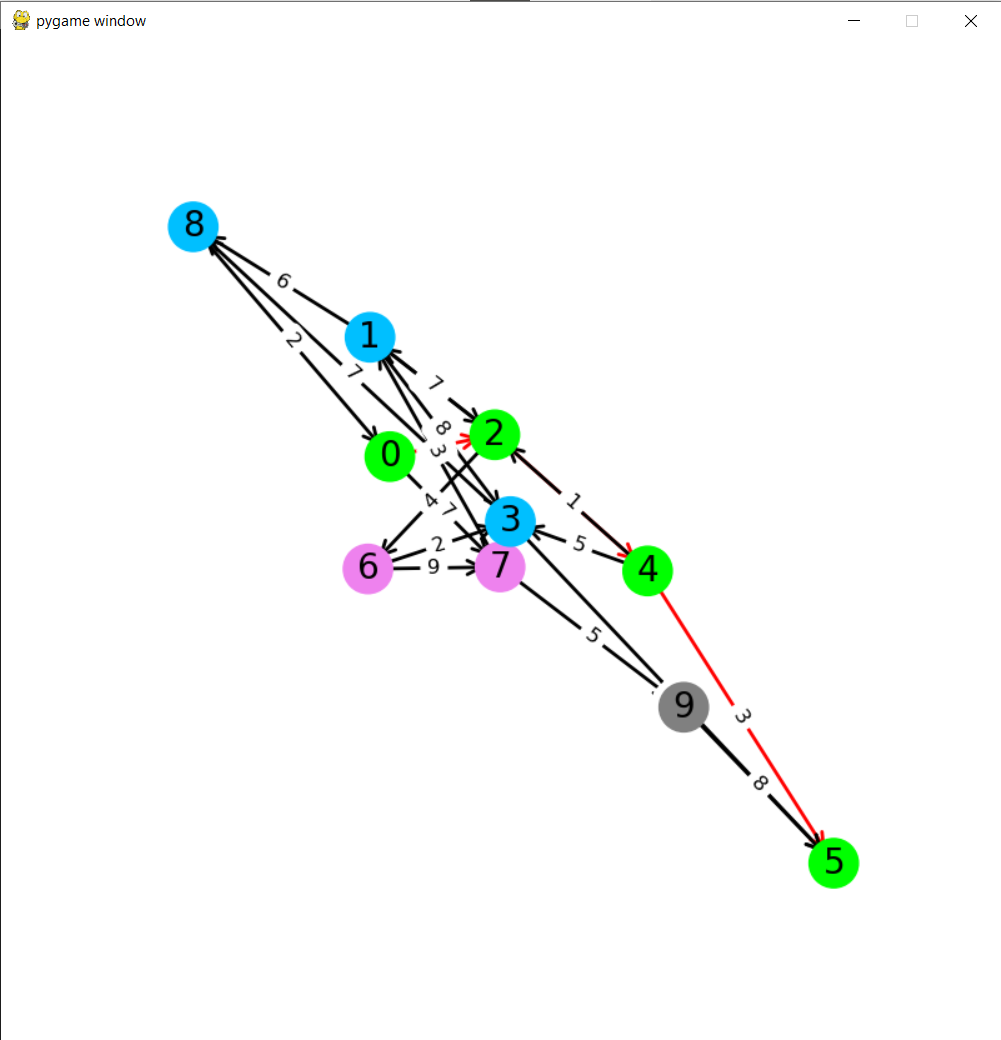
\includegraphics[width=0.5\textwidth]{result/testcase4/ids.png}
    \caption{IDS}
\end{figure}
\begin{figure}[h!]
    \centering
    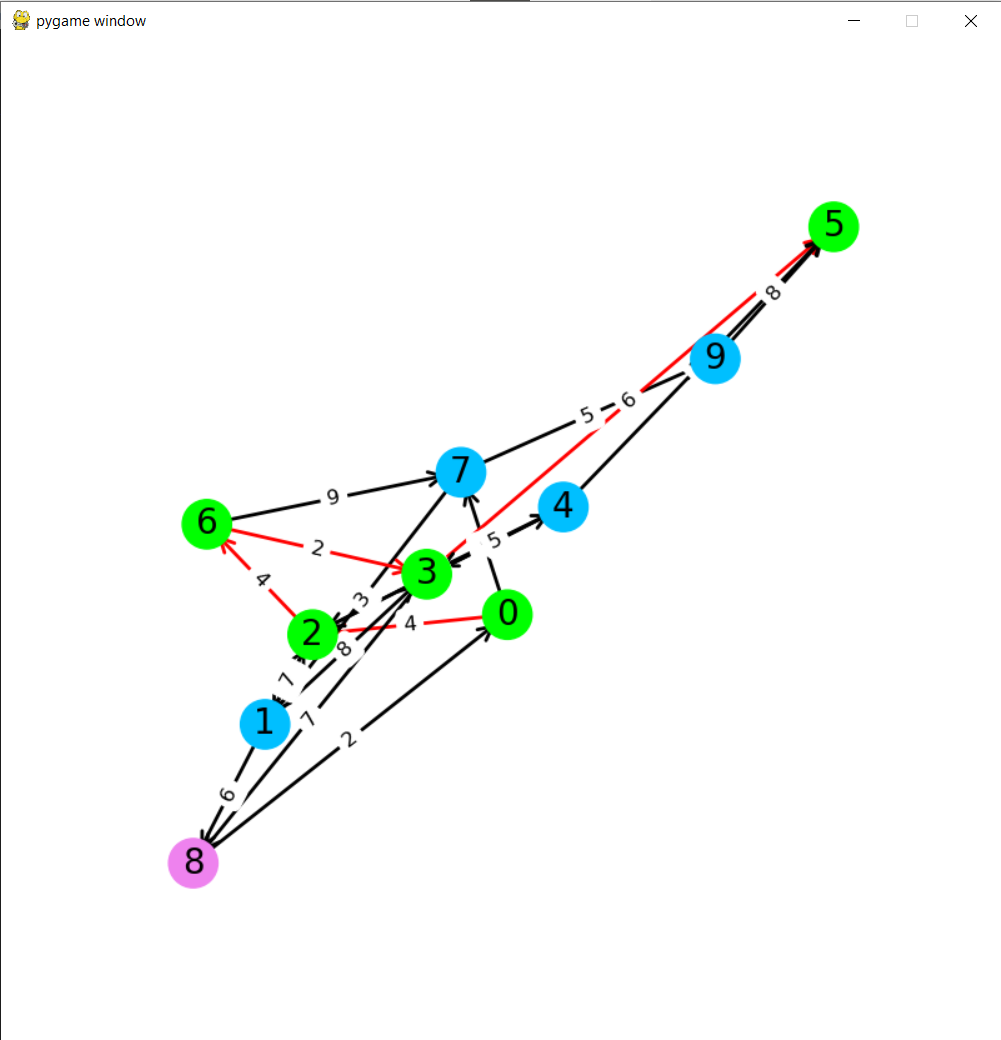
\includegraphics[width=0.5\textwidth]{result/testcase4/astar2.png}
    \caption{A* with Manhattan Distance}
\end{figure}
\clearpage

\subsubsection{test case 5}
\begin{figure}[h!]
    \centering
    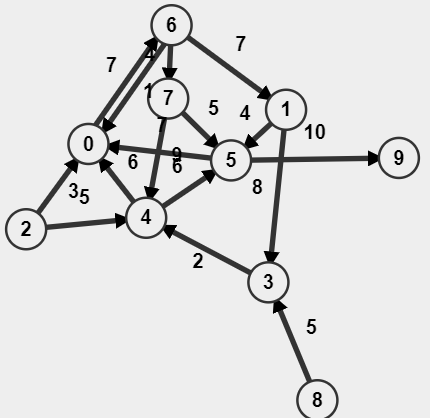
\includegraphics[width=0.5\textwidth]{testcase/5.PNG}
    \caption{Test Case 5 Image}
\end{figure}
\textbf{This is adjacency matrix for test case 5.}
\begin{verbatim}
2 9
0 0 0 0 0 0 7 0 0 0
0 0 0 8 0 4 0 0 0 0
3 0 0 0 5 0 0 0 0 0
0 0 0 0 2 0 0 0 0 0
6 0 0 0 0 6 0 0 0 0
7 0 0 0 0 0 0 0 0 10
1 7 0 0 0 0 0 4 0 0
0 0 0 0 9 5 0 0 0 0
0 0 0 5 0 0 0 0 0 0
0 0 0 0 0 0 0 0 0 0   
\end{verbatim}
\textbf{Test case Description:}
\begin{itemize}
    \item Number of nodes: 10 
    \item Number of edges: 20
    \item Start node: 2
    \item Goal node: 9
\end{itemize}

\paragraph*{Algorithm Results}

\quad The following are the results of the algorithms for test case 5.

\begin{figure}[h!]
    \centering
    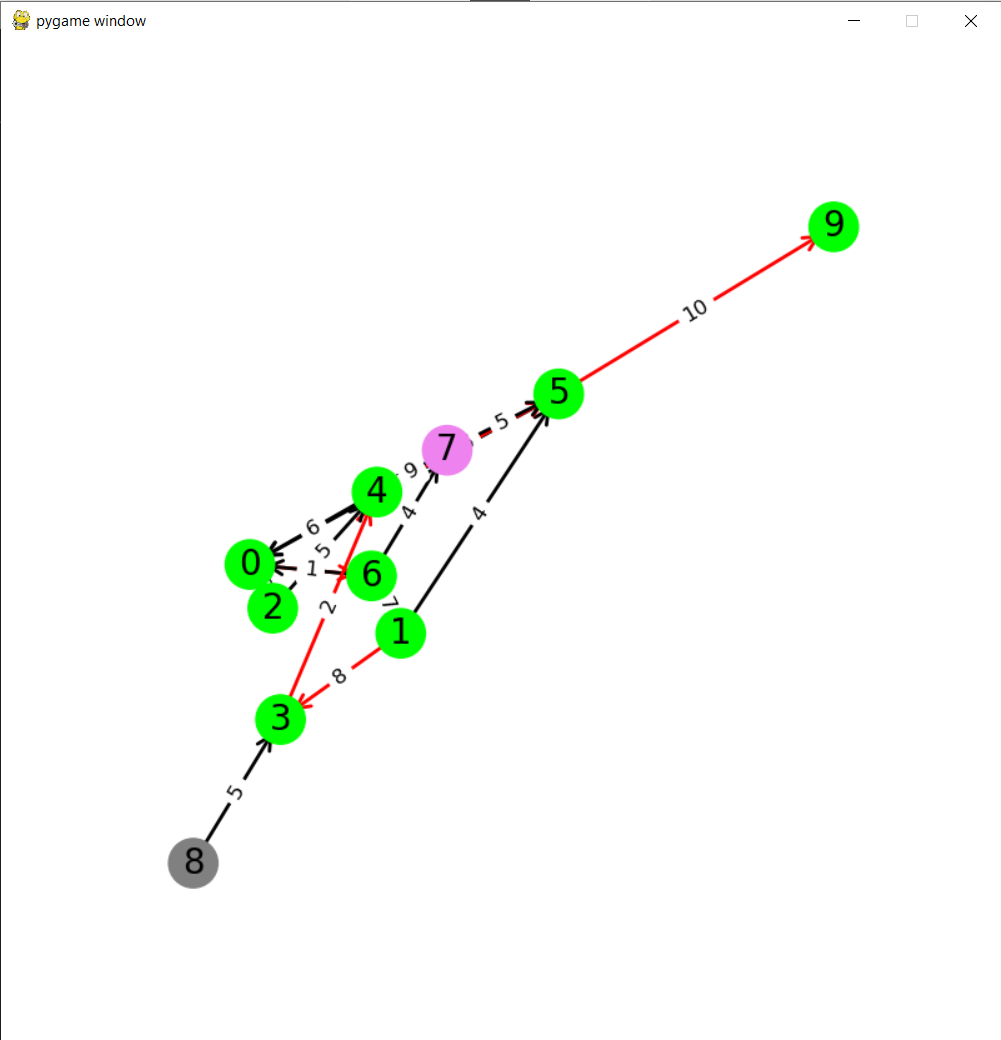
\includegraphics[width=0.5\textwidth]{result/testcase5/dfs.png}
    \caption{DFS}
\end{figure}
\begin{figure}[h!]
    \centering
    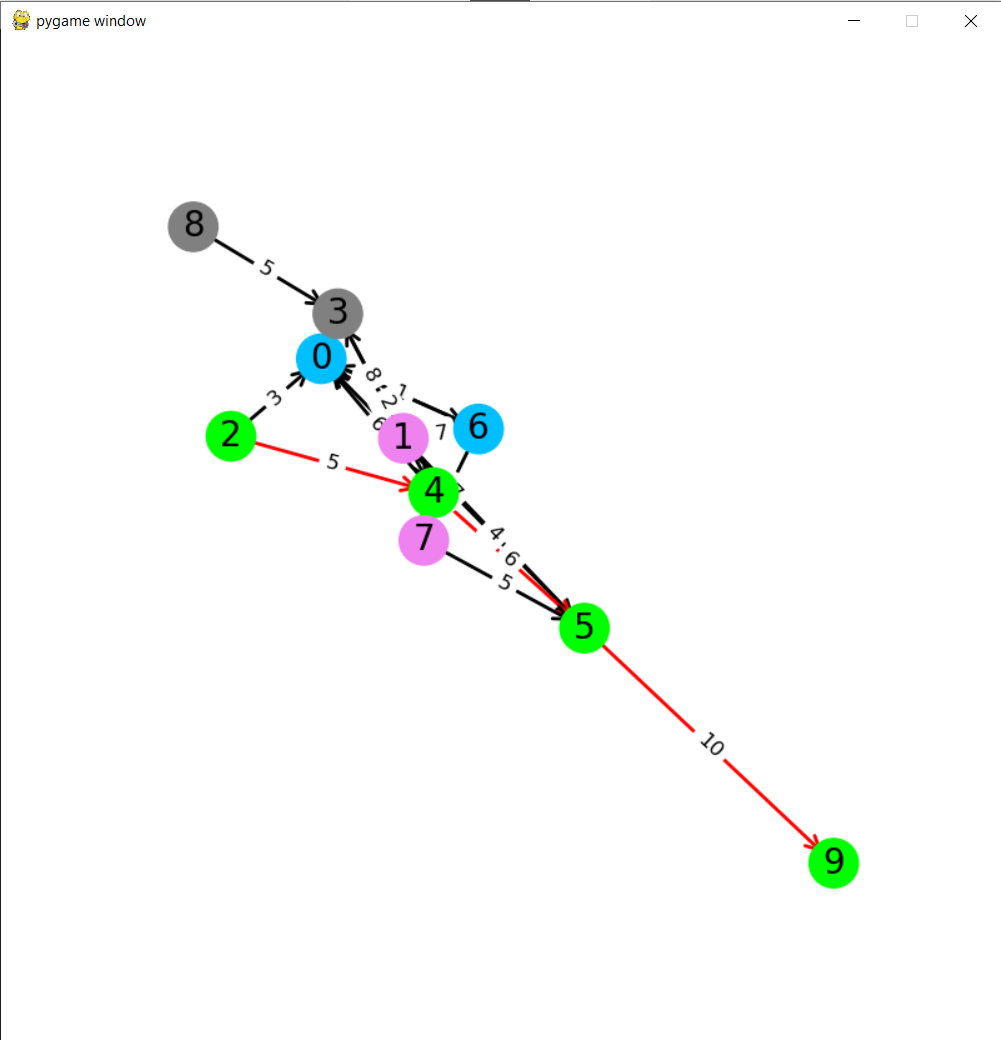
\includegraphics[width=0.5\textwidth]{result/testcase5/bfs.png}
    \caption{BFS}
\end{figure}
\begin{figure}[h!]
    \centering
    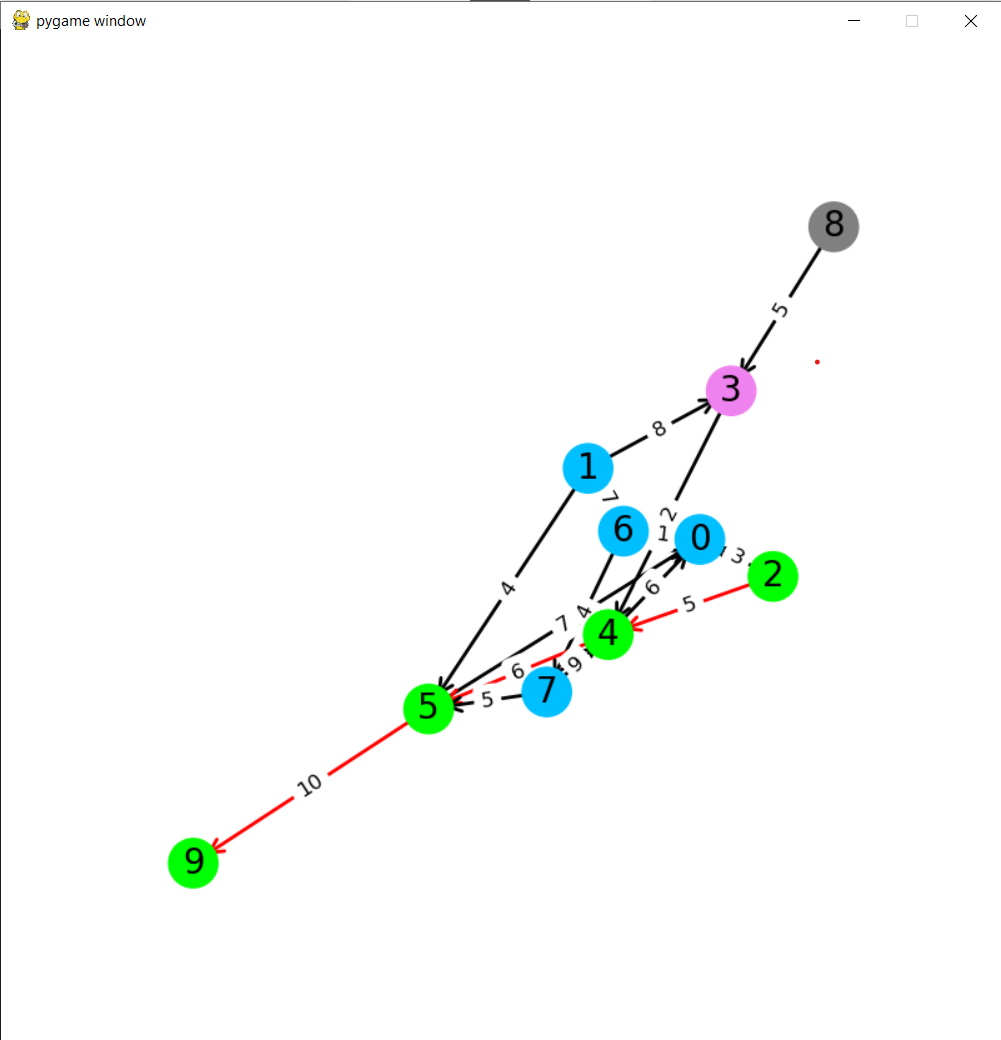
\includegraphics[width=0.5\textwidth]{result/testcase5/ucs.png}
    \caption{UCS}  
\end{figure}
\begin{figure}[h!]
    \centering
    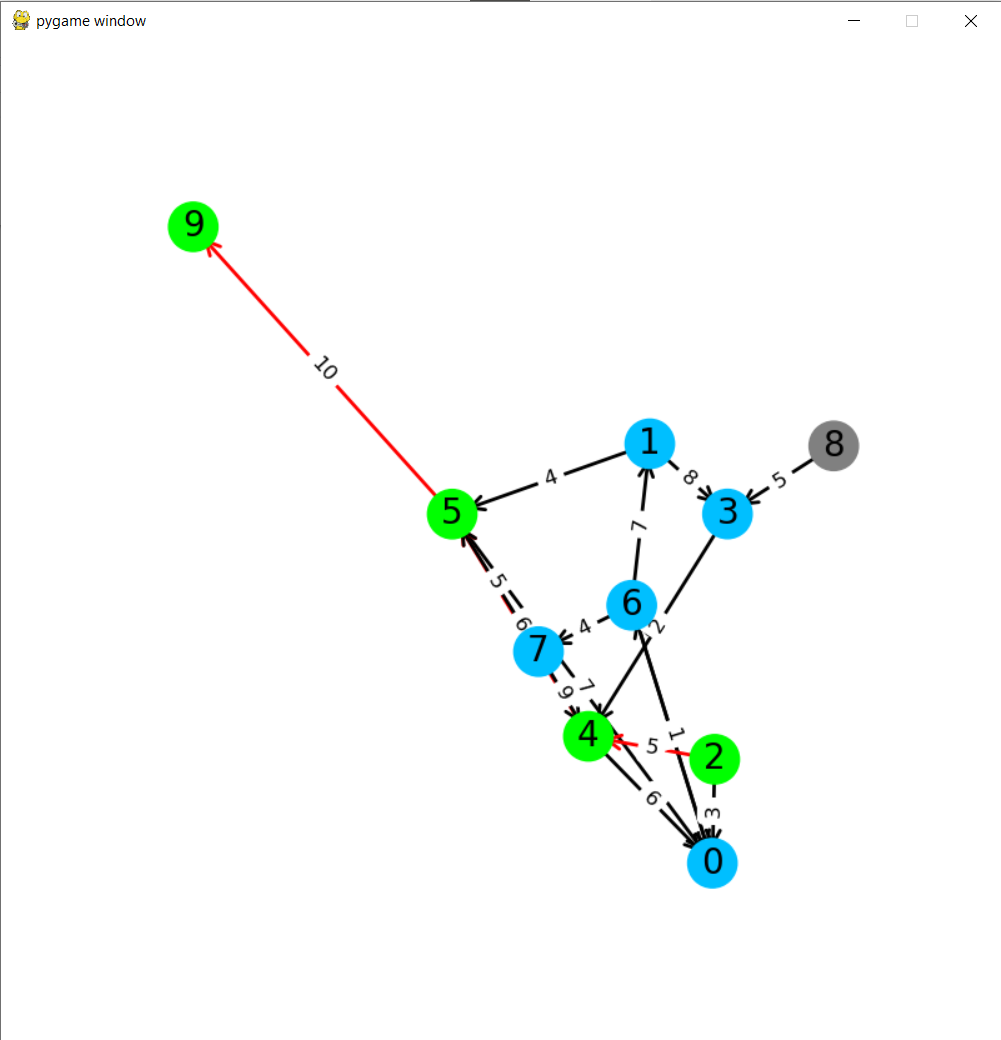
\includegraphics[width=0.5\textwidth]{result/testcase5/greedy.png}
    \caption{GBFS}
\end{figure}
\begin{figure}[h!]
    \centering
    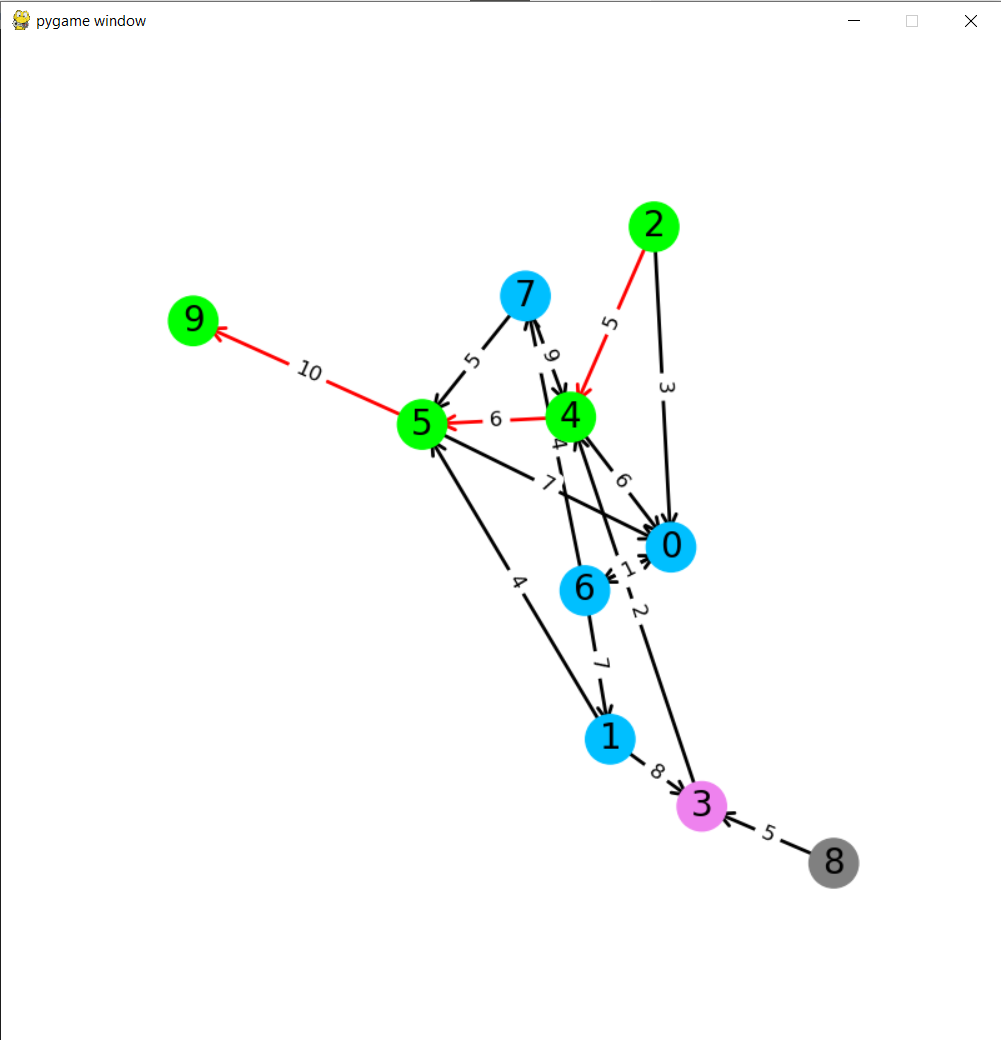
\includegraphics[width=0.5\textwidth]{result/testcase5/astar.png}
    \caption{A* with Euclidean Distance}
\end{figure}
\begin{figure}[h!]
    \centering
    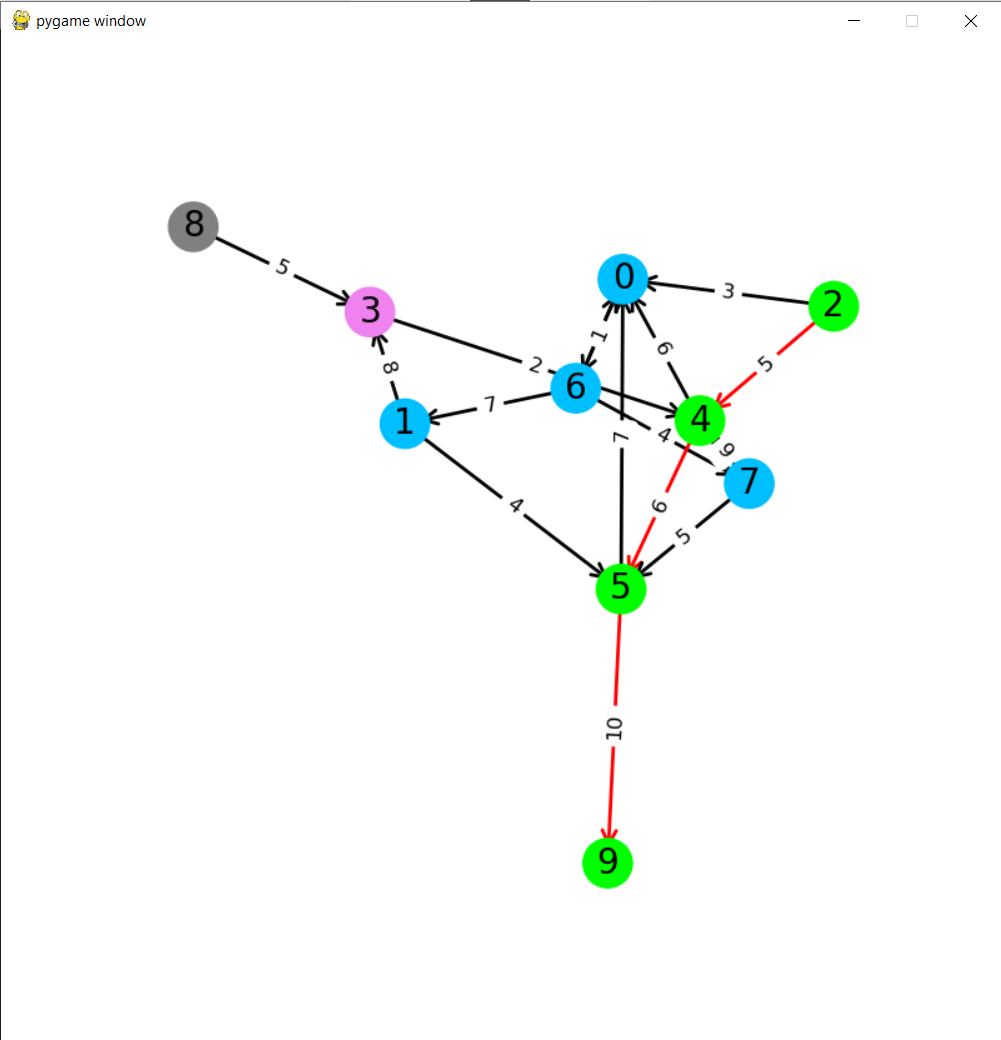
\includegraphics[width=0.5\textwidth]{result/testcase5/ids.png}
    \caption{IDS}
\end{figure}
\begin{figure}[h!]
    \centering
    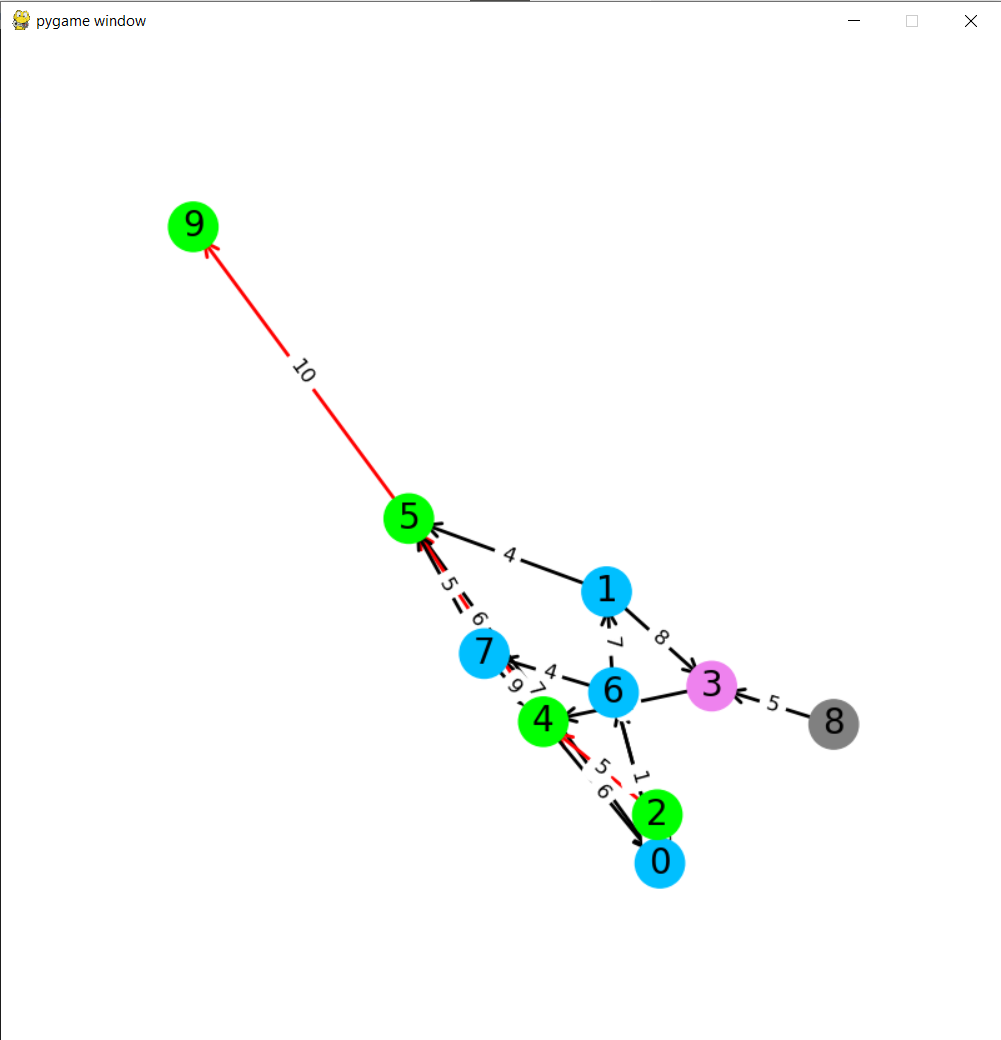
\includegraphics[width=0.5\textwidth]{result/testcase5/astar2.png}
    \caption{A* with Manhattan Distance}
\end{figure}
\clearpage

\pagebreak